
% ----------------------------
% Introducción.
% ----------------------------
\section*{Introducción}
En esta asignatura estudiaremos la geometría afín. Nos centraremos en el plano, el espacio y las figuras que se forman en él.
%%% TODO: completar introducción.
\newpage

\section{El espacio af\'in}
\begin{ndef}[Espacio af\'in]
  Sea $E$ un conjunto no vacío. Diremos que $E$ es un \textit{espacio afín} asociado a un espacio vectorial $V$ si existe una aplicación
  \begin{align*}
    \varphi: E \times E & \rightarrow V \\
    (a,b) & \mapsto \varphi(a,b)
  \end{align*}
  que cumpla las siguientes propiedades:
  \begin{nlist}
  \item Si fijamos un punto $a$, la aplicación $\varphi_a$ es biyectiva, o lo que es lo mismo:
    $$\forall a \in E, \ \ v \in V, \ \ \exists! \ b \in E:\varphi(a,b)=v$$
  \item Se tiene la relación de Charles, es decir:
    $$\forall a, b, c \in E \ \ \  \varphi(a,b) + \varphi(b,c) = \varphi(a,c)$$
  \end{nlist}
\end{ndef}
\subsection{El plano afín}

De ahora en adelante, en el desarrollo de estos apuntes consideraremos $\R^2$ como el plano afín. En este plano podemos representar tanto \textit{puntos} como \textit{vectores} (realmente lo haríamos en el plano vectorial). No vamos a entrar a detallar todas las propiedades de los vectores, que vamos a suponer que el lector conoce. \\

\begin{figure*}[h]
	\sffamily
  \centering
  \begin{tikzpicture}
	  	\draw[->] (-0.2,0) -- (4,0) node[right] {$x$};
  		\draw[->] (0,-0.2) -- (0,4) node[above] {$y$};
  		\node [fill=500, inner sep=1pt, scale=1.5, circle] at (2,3) {};
  		\draw [dashed, 300] (0,3) -- (2,3);
  		\draw [dashed, 300] (2,0) -- (2,3);
  		\draw[shift={(0,3)}] (2pt,0pt) -- (-2pt,0pt) node[left] {$3$};
  		\draw[shift={(2,0)}] (0pt,2pt) -- (0pt,-2pt) node[below] {$2$};
  \end{tikzpicture}
  \caption{El punto (2,3) en el plano}
\end{figure*}

Lo que vamos a tratar de hacer en este tema es \textit{transformar} las propiedades de los vectores en propiedades de puntos e intentar relacionar estos dos conceptos.

\begin{minipage}[b]{0.45\textwidth}
  Dados dos puntos $P$ y $Q$ del plano, podemos transformarlos en un vector llamando $\vec{u}$ al vector que une $P$ y $Q$. Así, $\vec{u} = \overrightarrow{PQ} = Q-P$. De forma analítica podemos observar también que si tenemos un punto $P$, podemos sumarle un vector $\vec{u}$ y obtenemos otro punto $Q$. Hemos visto entonces que podemos sumar tanto dos     vectores como puntos con vectores.
\end{minipage} \hfill
\begin{minipage}[b]{0.45\textwidth}
\begin{tikzpicture}
  \sffamily
  \tkzInit[ymin=-0.5,ymax=3.5,xmin=-0.5,xmax=5.5]
  \tkzAxeXY

  \tkzSetUpPoint[size=10,color=900, fill=700]

  \tkzDefPoint(0,0){O}
  \tkzDefPoint(1,1){P}
  \tkzDefPoint(2,2.5){Q}
  \tkzDefPoint(4,1){A}
  \tkzDefPoint(5,2.5){Ap}
  \tkzDrawPoints(P,Q)
  \tkzDrawPoints(A,Ap)

  \tkzDrawSegment[500, line width=1pt](P,Q)
  \tkzLabelPoints[below=0.5pt](P)
  \tkzLabelPoints[above=0.5pt](Q)
  \tkzLabelSegment[right=0.8em, pos=.4](P,Q){$\vec{u} = Q - P$}

  \tkzDrawSegment[500, line width=1pt](A,Ap)
  \tkzLabelPoints[below=0.5pt](A)
  \tkzLabelPoint[above=0.5pt](Ap){$A + \vec{u} = Q$}
  \tkzLabelSegment[right=0.8em, pos=.4](A,Ap){$\vec{u}$}


  %\tkzDrawSector[color=500, fill=50](O,A)(B)

  %\tkzText(1.25,1.25){$D$}
\end{tikzpicture}
\end{minipage}
\begin{ndef}[Combinación lineal de vectores]
  Si tenemos una familia $u_1,\ldots , u_n$ de vectores y $\alpha_1,\ldots, \alpha_n \in \R$ una familia de escalares, entonces a la expresión
  \[
    \sum_{i=1}^n \alpha_i u_i
  \]
  la llamamos \textit{combinación lineal de vectores}.
\end{ndef}

\begin{ndef}[Razón de vectores proporcionales]
  Dados $u$ y $v$ dos vectores proporcionales ($u = \lambda v$), llamamos \textit{razón} de esos dos vectores al escalar $\lambda \in \R$.
\end{ndef}

A continuación vamos a estudiar distintas \textit{combinaciones} de puntos del plano afín.

\begin{ndef}[Combinación baricéntrica de puntos]
  Dado $\{P_1,...,P_n\}$ un conjunto de puntos del plano afín y $\alpha_1,\dots,\alpha_n \in \R$ una lista de escalares que cumplan que $\sum_i \alpha_i = 1$, llamamos \textit{combinación baricéntrica de puntos} a:
  \[
    \sum_{i=1}^n \alpha_i P_i
  \]
  Los escalares $\alpha_1,\dots,\alpha_n$ se llaman \textit{pesos} de los puntos.
\end{ndef}

\begin{nprop} Una combinación baricéntrica de puntos es un punto.
\end{nprop}

\begin{proof}

  Sea $P = \sum_i \alpha_i P_i$ una combinación baricéntrica de puntos. Para simplificar la demostración, vamos a comenzar transformando los puntos en vectores.

  Restamos un punto cualquiera de la combinación como por ejemplo $P_1$, $P-P_1 = \sum \alpha_i(P_i-P_1)$, obteniendo así una identidad entre vectores de la forma:
  \[
    P-P_1 = \sum_{i=2}^n \alpha_i \overrightarrow{P_1P_i}
  \]

  Y llegamos a que
  \[
    P = P_1 + \sum_{i=2}^n \alpha_i \overrightarrow{P_1P_i}
  \]

  Hemos demostrado que $P$ es el resultado de sumar un vector a un punto (en este caso $P_1$), que es otro punto como queríamos.
\end{proof}

\begin{ndef}[Combinación convexa]
  Si en una combinación baricéntrica los pesos $\alpha_i$ asignados a los puntos son todos positivos, la llamaremos \textit{combinación convexa}. \end{ndef}

\begin{ndef}[Centro de gravedad de un conjunto de puntos]
  Si $\{P_1,\dots,P_n\}$ es un conjunto de puntos del plano afín y $\alpha_1,...,\alpha_n$ los \textit{pesos} asociados a estos puntos, llamamos a
  \[
    \sum_{i=1}^n \alpha_iP_i
  \]
  el \textit{centro de gravedad del conjunto de puntos}.
\end{ndef}

\begin{ndef}[Punto medio]
  Sean $P$ y $Q$ dos puntos en el espacio afín. Entonces definimos el punto medio entre $P$ y $Q$ como:
  \[
    M := \dfrac{1}{2} P + \dfrac{1}{2}Q = \dfrac{1}{2}(P+Q)
  \]
  Alternativamente, si $u = \overrightarrow{PQ}$, entonces:
  \[
    M = \dfrac{1}{2}u + P
  \]

\end{ndef}

\subsection{Sistemas de referencia y coordenadas}

\begin{ndef}[Sistema de referencia]
Sea $V$ un espacio vectorial de dimesión finita y $E$ un espacio afín asociado a $V$. Llamaremos \textit{ sistema de referencia cartesiano } a cada conjunto $R=\{O,B\}$ donde $O\in E$ y $B$ es base de $V$.

$O$ se denomina el origen del sistema de referencia

\end{ndef}

Entonces $\forall A \in E$, las cordenadas de $A$ respecto de R se definen como las coordenadas del vector $\vec{OA}$ respecto de $B$. Es decir, si $B] = v_1, ... ,v_n $ y $\vec{OA} = \sum_{i=1}^{n} a_i*v_i$, entonces $A = (a_1,..., a_n)$.

\begin{ndef}[Sistema de referencia ortogonal]
Sea $V$ un espacio euclídeo, $E$ un espacio afín asociado a $V$ y $R=\{O,B\}$ un sistema de referencia, diremos que $R$ es ortogonal si B es ortonormal.

\end{ndef}

En este caso se induce en $E$ una distancia como $d(A,B) = \|\vec{AB}\|\ \forall A,B \in E$

%%%No tengo del todo claro si ponerlo como teorema o como si nada, pues la propia demostración esta implícita en el enunciado.
%\begin{nth}

%Sea $E$ el espacio afín asociado a $V=L(B)=L(B')$, sean $O,O'\in E$ y a partir de estos $R=\{O,B\}$ y $R'=\{O',B'\}$.

%Sea $M(1_V,B',B)$ la matriz de cambio de base de $B'$ a $B$. Notaremos para esta fórmula $\vec{OA}=A_R$, $\vec{OO'}=O'_R$ y $\vec{O'A}=A_{R'}$ evidenciando así la relación entre las coordenadas de los vectores respecto a las bases y las coordenadas de los puntos respecto a los sistemas de referencia. De esta forma tenemos que:

%$$\vec{OA}=\vec{OO'}+\vec{O'A}=\vec{OO'}+M(1_V,B',B)\vec{O'A}$$

%luego $A_R=O'_R+M(1_V,B',B)A_{R'}$.

%\end{nth}


\subsection{Rectas afines}

En este apartado vamos a describir las \textit{rectas afines}. De ahora en adelante, si se hace mención a una recta sin más, daremos por hecho que se trata de una recta afín.

\begin{ndef}[Recta vectorial]
  Una recta vectorial es un subespacio vectorial de dimensión $1$, es decir, para generarla es necesario un único vector. Podemos denotar la recta vectorial generada por un vector $v$ como $L(v)$.
\end{ndef}

\begin{ndef}[Recta afín]
  Si $P$ es un punto y $v$ un vector, entonces una recta afín $r$ viene dada por
  \[
    r = P+L(v) = \{P + \lambda v : \lambda \in \R\}
  \]
  Para distinguir las rectas vectoriales de las rectas afines, notaremos a $L(v)$ como $\vec{r}$.
\end{ndef}

\begin{ndef}[Variedad de dirección]
  Si $r$ es una \textit{recta afín}, llamaremos \textit{variedad de dirección de r} a $\vec{r}$.
\end{ndef}

\begin{nprop}[Propiedades de las rectas afines]\hfill
\begin{nlist}
\item Si $Q$ es un punto y $r$ una recta tales que $Q\in r \implies r = Q +L(v)$ donde $v$ es el vector director de la recta $r$.
\item Si $P,Q$ son dos puntos, entonces por ellos pasa una única recta $r = P +L(\overrightarrow{PQ})$. \\

\end{nlist}
\end{nprop}

 \begin{proof} \hfill

 \begin{nlist}
	\item Es obvio que dado $r = \{P+\lambda v : \lambda \in \mathbb{R}\},$ este conjunto es identico a $r = Q +L(v)$, puesto que al estar tanto $P$ como $Q$ en $r$, $\vec{PQ}$ es proporcional a $v$

\item (Existencia) $r$ es una recta y es trivial por su definición que contiene tanto a $P$ como a $Q$.

    (Unicidad) Si la recta $r$ pasa por $P$ y $Q$ y sea $s$ otra recta que pasa por ellos, entonces es consecuencia directa de la definición que:
    \[
      s = P+L(\overrightarrow{PQ}) = r
    \]


\end{nlist}
  \end{proof}

\subsubsection{Posición relativa entre rectas}

Podemos clasificar un par de rectas $r$ y $s$ por su posición en el plano afín. Así, decimos que dos rectas son

\begin{itemize}
\item Paralelas, notado $r\parallel s$, si y solo si $\vec{r} = \vec{s}$
\item No paralelas, notado $r\nparallel s$, si y solo si sus vectores directores son linealmente independientes o lo que es lo mismo, $u$ y $v$ forman una base.
\end{itemize}

\begin{nth}
  Sean $r$ y $s$ dos rectas del plano afín. Entonces:
  \begin{nlist}
  \item $r \nparallel s\implies r \cap s = A$, un punto
  \item $r \parallel s \implies r = s$ o bien $r \cap s =  \emptyset$
  \end{nlist}
\end{nth}
  \begin{proof}\hfill\\
    \begin{nlist}
      % REVIEW: No acabo de ver que demuestre lo que dice (i)
    \item Si $u,v$ son los vectores directores de $r$ y $s$ y $P$ y $Q$ puntos de $r$ y $s$ respectivamente, entonces con los pares $\{u,v\}$ tenemos que $P+\lambda u = Q + \mu v$ con $\lambda, \mu \in \R$
      y si $r = P +L(u)$ y $s=Q+L(v)$, y $\overrightarrow{PQ} = \lambda u - \mu v $ y, por ello, existen únicos $\lambda, \mu$.
    \item Sean $u,v$ los vectores directores de $r$ y $s$. Supongamos que además tienen al menos un punto $A$ en común. Escribimos estas rectas como $r = A +L(u)$ y $s=A+L(v)$. Como $r \parallel s \implies L(r)=L(s)$ descubrimos que $r = A +L(u)=A+L(v) = s$.
   	%TODO: demostrar que cuando no existe el punto A la intersección es vacía
    \end{nlist}
  \end{proof}


\subsection{Triángulos}
Los \textit{triángulos} son polígonos que vienen dados por tres puntos no alineados $A, B, C$ llamados \textit{vértices} y las tres rectas que los unen.

\begin{ndef}[Coordenadas baricéntricas en un triángulo]
	Si $ABC$ es un triángulo en $\R^2$, cualquier punto interior a él puede ser representado por tres coordenadas $(\alpha,\beta,\gamma)$ baricéntricas tales que:
	\[
	\alpha + \beta + \gamma = 1 \quad \text{con } 0\leq \alpha,\beta,\gamma \leq 1
	\]
	Donde la relación entre las coordenadas cartesianas y las baricéntricas viene dada por:
	\[
	\begin{cases}
	x = \alpha x_A + \beta x_B + \gamma x_C\\
	y = \alpha y_A + \beta y_B + \gamma y_C
\end{cases}
	\]
\end{ndef}


\begin {ndef}
  Dos o más puntos $A_1, A_2, ... , A_n $ están alineados $\iff$ existe una recta $r \subset \mathbb{R}^2$ tal que $A_i \in r\ \forall i \in 1,...,n$
\end{ndef}


\begin{nprop}
  $A,B,C$ son puntos no alineados  $ \iff \overrightarrow{AB}, \ \overrightarrow{AC}$ son linealmente independientes.
\end{nprop}

  \begin {proof}\hfill\\
    \boxed{\Rightarrow}
    Si los puntos $A$, $B$, y $C$ no están alineados entonces $\nexists r \subset \mathbb{R}^2$ una recta tal que $A$, $B$, y $C \in r$, luego $\nexists \vec{v}$ tal que $A,B,C \in r = A + L(\vec{v})$. Por tanto, $\overrightarrow{AB} \neq \alpha \cdot \overrightarrow{AC}, \alpha \in \mathbb{R}\ $ porque si no, sería cierto lo anterior. Así, $\overrightarrow{AB}$ y $\overrightarrow{AC}$ son linealmente independientes.

    \boxed{\Leftarrow} Si $A$, $B$ y $C$ están en la misma recta, entonces la única recta que une puntos A y B y los puntos los A y C es la misma, luego $r = A + L(\overrightarrow{AB})  = A + L(\overrightarrow{AC})$, por lo que $\overrightarrow{AB}$ y $\overrightarrow{AC}$ serían linealmente dependientes. Como sabemos que $\overrightarrow{AB}$ y $\overrightarrow{AC}$ no lo son, A, B y C no están alineados.
  \end{proof}

\begin{nth}\hfill\\
\begin{minipage}[c]{0.50\textwidth}
  \hfill\\
  Se consideran los triángulos $ABC$ y $A_1B_1C_1$. Si dos lados de $ABC$ son paralelos con sus homólogos de $A_1B_1C_1$ y las razones de sus vectores directores son iguales, los lados homólogos restantes también son paralelos y su razón, igual a la de los lados anteriores.
\end{minipage}\hfill
\begin{minipage}[]{0.47\textwidth}
  \begin{tikzpicture}[scale=.8]
  \sffamily
  % Definimos los vértices
  \tkzDefPoint(0,0){A}
  \tkzDefPoint(0,3){B}
  \tkzDefPoint(4,0){C}
  \tkzDefPoint(-2,0){A1}
  \tkzDefPoint(-2,4.5){B1}
% Dibujamos el rectángulo
\tkzDrawPolygon[color=500, fill=50](A1,B1,C)
\tkzDrawPolygon[color=500, fill=50](A,B,C)

% Dibujamos las diagonales
%\tkzDrawSegment[color=300, dashed](A,C)
%\tkzDrawSegment[color=300, dashed](B,D)

% Configuramos el estilo de los puntos
\tkzSetUpPoint[size=10,color=900, fill=700]

% Dibujamos los puntos
\tkzDrawPoints(A, B, C, A1, B1)
\tkzLabelPoints[above=.5em](B)
\tkzLabelPoints[below=.5em](A)
\tkzLabelPoints[below left=.5em](A1)
\tkzLabelPoints[above left=.5em](B1)
\tkzLabelPoint[below right](C){$C = C_1$}

\end{tikzpicture}
\end{minipage}

  \end{nth}

  %FIXME: Corregir esta demostración, no está bien explicada.
  \begin{proof}
    Si los lados son paralelos, entonces los vectores directores son proporcionales.
    Si $w$ (el lado no mencionado del primer triángulo) es $w=-u+v$ y $w_1$(el lado no mencionado del segundo triángulo) es $w_1 = - \lambda u + \lambda v = \lambda (-u+v) = \lambda w$  por lo que tenemos lo que queríamos.
  \end{proof}

\begin{ndef}[Triángulos semejantes]
  Dos triángulos son semejantes si sus lados son paralelos dos a dos. También son semejantes $\iff$ los ángulos son iguales. También son semejantes si sus lados son proporcionales.
\end{ndef}

\begin{ncor}[Teorema de Thales]
  Si en un triángulo $ABC$ se traza una recta paralela a cualquiera de sus lados, obtenemos un triángulo semejante al triángulo original.
\end{ncor}

\begin{nota}
  Dos triángulos tienen todos los lados paralelos dos a dos $\iff$ los segmentos de los lados son proporcionales dos a dos. Esto es por el teorema anterior.
\end{nota}

\begin{ndef}[Triángulo medio]
  Si $ABC$ es un triángulo, sus puntos medios $A'$, $B'$ y $C'$ forman el \textit{triángulo medio}.
\end{ndef}

\begin{nprop}
  Los lados homólogos de un triángulo en su triángulo medio tienen razón $-\frac{1}{2}$.
\end{nprop}

\begin{proof}
  Tenemos que: $A' = B/2 + C/2$, $B' = A/2+C/2$, $C' = A/2 + B/2$. Tenemos por tanto que: $\vec{A'B'} = B'-A' = \dfrac{1}{2}(A-B) = -\dfrac{1}{2} \vec{AB}$ y por tanto los lados homólogos son paralelos.

      Además, el factor es el número obtenido en la conversión, es decir $-\dfrac{1}{2}$.
\end{proof}

%% Centros y ejes de un triangulo
\subsubsection{Centros y ejes de un triángulo}

\begin{ndef}[Medianas de un triángulo]

  Las medianas de un triángulo $ABC$ son las rectas que unen un vértice con el punto medio del lado opuesto

\end{ndef}
\begin{ndef}[Baricentro de un triángulo] \hfill\\
  \begin{minipage}[c]{0.70\textwidth}
  El baricentro $G$ de un triángulo es un punto que viene dado por:
  \[
    G = \dfrac{1}{3} A +  \dfrac{1}{3} B +  \dfrac{1}{3} C
  \]
  \end{minipage}
  \begin{minipage}[]{0.27\textwidth}
    \pgfdeclarelayer{0}
\pgfdeclarelayer{1}
\pgfdeclarelayer{2}
\pgfdeclarelayer{3}
\pgfsetlayers{0,1,main,2,3}

\begin{center}
  \sffamily
  \begin{tikzpicture}[scale=1.5]
    \begin{pgfonlayer}{3}
      \coordinate [label=left:$A$] (A) at (0,0);
      \coordinate [label=right:$B$] (B) at (2,0);
      \coordinate [label=above:$C$] (C) at (1,2);
    \end{pgfonlayer}{3}
    \begin{pgfonlayer}{1}
      \draw [500, fill=50] (A) -- (B) -- (C) -- cycle;
    \end{pgfonlayer}{1}
    \begin{pgfonlayer}{3}
      \node [fill=700,inner sep=1pt,label=below:$M_{AB}$, scale=1.5, circle] (MAB) at
      ($ (A)!.5!(B)$) {};
    \end{pgfonlayer}{3}
    \coordinate (C1) at ($ (MAB)!1.2!(C)$);
    \coordinate (C2) at ($ (MAB)!-.3!(C)$);
    \draw [dashed, 700, name path=MC](C1) -- (C2);
    \begin{pgfonlayer}{3}
      \node [fill=700,inner sep=1pt,label=left:$M_{AC}$, scale=1.5, circle] (MAC) at ($
      (A)!.5!(C)$) {};
    \end{pgfonlayer}{3}
    \coordinate (B1) at ($ (MAC)!1.2!(B) $);
    \coordinate (B2) at ($ (MAC)!-.3!(B)$);

    \draw [dashed, 700, name path=MB] (B1) -- (B2);

    \begin{pgfonlayer}{3}
      \node [fill=orange,inner sep=1pt,label=right:$M_{BC}$, scale=1.5, circle] (MBC) at ($
      (B)!.5!(C)$) {};
    \end{pgfonlayer}{3}
    \coordinate (A1) at ($ (MBC)!1.2!(A) $);
    \coordinate (A2) at ($ (MBC)!-.3!(A)$);

    \draw [dashed, 700] (A1) -- (A2);

    \path [name intersections={of=MB and MC, by=G}];
    \begin{pgfonlayer}{3}
      \node [fill=700, inner sep=1pt, label=below:$G$, scale=1.5, circle] at (G) {};
    \end{pgfonlayer}{3}
  \end{tikzpicture}
\end{center}

  \end{minipage}
\end{ndef}

\begin{nth}
  Si $ABC$ es un triángulo en el plano afín, entonces las medianas son concurrentes. Su punto de corte es el baricentro $(G)$. El baricentro triseca el segmento que une un vértice con el punto medio homólogo.


\end{nth}

\begin{proof}
  Sea $A'$ el punto medio del lado opuesto a $A$ en un triángulo $ABC$. Sea $A \vee A'$ una de las medianas. Esta es:
  \[
    \{\lambda A + \mu A': \lambda, \mu \in \R \text{ , } \lambda+\mu = 1\}
  \]
  Sabemos que $G = \dfrac{1}{3} A +  \dfrac{1}{3} B +  \dfrac{1}{3} C$ y queremos ver si está en la mediana. Lo que queremos comprobar es que:
  \[
    G = \dfrac{1}{3} A +  \dfrac{1}{3} B +  \dfrac{1}{3} C = \lambda A + \mu A'
  \]

  Es claro que $A' = \left(\frac{1}{2}B + \frac{1}{2}C\right)$. Tomamos $\lambda = \frac{1}{3}$, por lo que $\mu = \frac{2}{3}$ ya que el punto que buscamos se encuentra en la mediana. Sustituyendo estos valores en la ecuación anterior:

  $$\dfrac{1}{3}A + \dfrac{2}{3}\left(\dfrac{1}{2}B+\dfrac{1}{2}C\right) = \frac{1}{3}A + \frac{1}{3}B + \frac{1}{3}C = G$$
	Después, una vez que sabemos que este punto se encuentra en la recta en la recta que une el punto medio con su vértice homólogo, como este se expresa como un tercio del vértice más otros dos puntos no alineados, este punto triseca claramente a ese segmento.
\end{proof}

\begin{nota}
  A partir de ahora, usaremos $\mu(A,B)$ para denotar la distancia euclídea entre los puntos $A$ y $B$.
\end{nota}

\begin{ndef}[Mediatriz de un segmento] \hfill\\
\begin{minipage}[c]{0.70\textwidth}
  Si $\overline{AB}$ es un segmento, entonces llamamos $m_{AB}$  al lugar geométrico $\mathcal{L}=\{P \in \R^2 : \mu(AP) = \mu(BP)\}$ (los puntos del plano que distan lo mismo que A que de B).
\end{minipage}
\begin{minipage}[]{0.27\textwidth}
  \begin{center}
  \sffamily
  \begin{tikzpicture}
    \coordinate [label=left:$A$] (A) at (0,0);
    \coordinate [label=right:$B$] (B) at (2,0.5);
    \draw[700] (A) -- (B);
    \coordinate (M) at ($ (A)!.5!(B)$);
    \coordinate (top) at ($ (M) !1! 90:(B)$);
    \coordinate (bottom) at ($ (M) !1! 270:(B)$);
    \draw [dashed, 500] (top) -- (bottom) node[right] {$m_{AB}$};
  \end{tikzpicture}
\end{center}
\end{minipage}
\end{ndef}

\begin{nprop}\hfill
  \begin{nlist}
    \item El punto medio $M \in \mathcal{L}$.
    \item La mediatriz es una recta que viene dada por $\langle\vec{AB},P\rangle  = \dfrac{1}{2}(|B|^2-|A|^2)$ y que es perpendicular al segmento $\overline{AB}$ y pasa por $M$ el punto medio del segmento.
  \end{nlist}
\end{nprop}

\begin{proof}\hfill
  \begin{nlist}
    \item Trivial.
    \item La mediatriz está dada por $\mathcal L = \{P\in\mathbb{R}^2, \mu(P,A) = \mu(P,B)\iff \mu(P,A)^2 = \mu(P,B)^2\}$. Sea $P(x,y),A(x_1,y_1),B(x_2,y_2)$, entonces $\mu(P,A)^2 = |P|^2+|A|^2-2\langle A,P\rangle  = |P|^2+|B|^2-2\langle B,P\rangle = \mu(P,B)^2 \implies$ $$ \frac{|A|^2-|B|^2}{2} =\langle A-B,P\rangle  = \langle\vec{BA},P\rangle $$
    Donde podemos ver que $\frac{|A|^2-|B|^2}{2}$ es una constante y $\langle\vec{BA},P\rangle $ genera la recta:
    \[
      r: \vec{BA}_1x+ \vec{BA}_2y - \frac{|A|^2-|B|^2}{2} = 0
    \]
    donde $\vec{BA}_i$ es la coordenada $i$-ésima del vector $\vec{BA}$ y por lo tanto $r$ es perpendicular a $\vec{BA}$.
  \end{nlist}
\end{proof}

\begin{nota}
  $|\vec{AP}|^2 = \mu(A,P)^2\implies \mu(A,P)^2 = 	\left(\sqrt{\langle \vec{AP},\vec{AP}\rangle }\right)^2 =  \langle A-P, A-P \rangle  =^{(1)} \langle A,A-P\rangle -\langle P,A-P\rangle  =  \langle A,A\rangle  - \langle A,P\rangle +\langle P,P\rangle - \langle P,A\rangle   = |A|^2+|P|^2-2 \langle P,A\rangle $. Y en (1) hemos aplicado la bilinealidad del producto escalar.
\end{nota}
\begin{ndef}[Rectas perpendiculares.]
  Dos rectas son perpendiculares si sus vectores directores son ortogonales.
\end{ndef}

\begin{ndef}[Mediatrices de un triángulo]
  Si $ABC$ es un triángulo, cada lado de este triángulo tendrá su mediatriz. Por tanto, tendremos 3 mediatrices para cada triángulo.
\end{ndef}

\begin{nth}
  Las tres mediatrices de un triángulo son concurrentes. Además, concurren en el punto $O$ llamado el circuncentro, el centro de la circunferencia que pasa por $A$,$B$ y $C$.
\end{nth}
\begin{proof}
  Sabemos que dos mediatrices nunca son paralelas. Tomemos $O$ como el único punto tal que $O \in  m_{AB} \cap m_{AC}$. Por la definición de mediatriz tenemos que $\mu(AO) = \mu(BO)$ y que $\mu(AO) = \mu(CO)$. Es obvio entonces que $\mu(BO) = \mu(CO)$ luego $O \in m_{BC}$.

\end{proof}

\begin{ndef}[Alturas de un triángulo]
  Son las rectas que pasan por un vértice y son perpendiculares al lado opuesto del triángulo. Estas alturas se cortan en el ortocentro $H$.
\end{ndef}

\begin{nota}
  Las mediatrices de un triángulo $ABC$ son las alturas de $A'B'C'$, por lo que las alturas de $A'B'C'$ son concurrentes.
\end{nota}

\begin{nprop}
  Todo triángulo $ABC$ es el triángulo medio de otro triángulo $A''B''C''$
\end{nprop}
\begin{proof}
  Para ello, tenemos que considerar $A'' = C+ \vec{AB}$. Ídem con $B''$ y $C''$.
\end{proof}

\begin{ndef}
  El triángulo doble $DEF$ de un triángulo $ABC$ es el triángulo tal que $ABC$ es el triángulo medio de $DEF$.
\end{ndef}

\begin{nota}
  Todo triángulo $ABC$ tiene un triángulo doble asociado, el cual es el hallado en la proposición anterior.
\end{nota}

\begin{nprop}
  Si $ABC$ es un triángulo y $A'B'C'$ su triángulo medio, entonces las alturas de $A'B'C'$ son las mediatrices de $ABC$ y $O=H'$
\end{nprop}
\begin{proof}
  Si tomamos $m_{BC}$ sabemos que pasa por $A'$ y es perpendicular a $\vec{BC}$, por lo que es perpendicular a $\vec{B'C'}$, por lo que será la altura del triángulo medio que pasa por $A'$. Análogamente ocurre con los $B'$ y $C'$, por tanto, $O=H'$.
\end{proof}


\begin{nprop}Si 2 de los centros del triángulo ABC coinciden, entonces el triángulo es equilátero.
\end{nprop}

%\begin{proof}
%	Si es equilátero $\implies$ coinciden todos los centros, por lo que veremos que si no es equilátero no coinciden.
%	Supongamos que no es equilatero, entonces
%\end{proof}

\begin{ndef}[Homotecia]
  Se define homotecia de centro $A$ y razón $\lambda$ como la aplicación $h_{A,\lambda}(P) = \lambda P + (1-\lambda)A = A+\lambda(\vec{AP})$
\end{ndef}

\begin{nprop} Si $h$ es una homotecia de razón $\lambda\ne 0$, entonces
\begin{enumerate}
\item $h$ multiplica la distancia por $|\lambda|$.
\item $h$ lleva rectas perpendiculares en rectas perpendiculares.
\item $h$ lleva mediatrices en mediatrices.
\item $h$ lleva alturas en alturas.
\end{enumerate}
\end{nprop}

\begin{proof}\hfill
\begin{enumerate}
	\item $h(P)-h(Q)=(A+\lambda(\vec{AP})) -(A+\lambda(\vec{AQ})) = \lambda(A-P) - \lambda(A-Q) = \lambda (Q-P)$.
	\item  Sean $r$ y $ s$, rectas perpendiculares, $P,P' \in r$ y $Q,Q'\in s$ puntos de las rectas. $\langle h(P) - h(P'),h(Q) - h(Q')\rangle  =  \langle \lambda (\vec{PP'}), \lambda(\vec {QQ'})\rangle=^1 \lambda^2 \langle \vec{PP'},\vec{QQ'}\rangle  = \lambda^2 \cdot 0 = 0 $, donde en 1 se ha usado la bilinealidad del producto escalar.
	\item Si $h$ multiplica distancia por $\lambda$, las distancias iguales siguen siendo iguales, por lo que el conjunto de puntos que están a la misma distancia de dos rectas se mantiene.
	\item Como $h$ lleva distancias iguales en distancias iguales, mantiene puntos medios. Además al mantener perpendicularidad, la recta perpendicular que pasa por el punto medio se mantiene.
\end{enumerate}
\end{proof}


\begin{nprop}

Para toda homotecia, el centro, un punto y su imagen están alineados.
\end{nprop}

\begin{proof}
	Sea la homotecia $h_{A,\lambda}(P) = \lambda P + (1-\lambda)A = A+\lambda(\vec{AP})$ y el punto cualquiera $P$. Veamos que en la recta (única) que contiene a $P$ y a $ A$, $r= A + \mu \vec{AP}$,  contiene a $h_{A,\lambda} (P)$. Esto es obvio por la misma definición de homotecia.
\end{proof}


\begin{nth}[Recta de Euler]
  Dado un triángulo $ABC$ no equilátero, entonces sus tres centros $G,O,H$ están alineados en la recta de Euler. Además $G$ triseca al segmento $\overrightarrow{OH}$.
\end{nth}
\begin{proof}
  Tomamos el triángulo y su triángulo medio $A'B'C'$. Entonces, hay una homotecia ($h$) de centro $G$ y razón $\dfrac{-1}{2}$ que lleva $ABC$ en $A'B'C'$ (probarlo aplicando la fórmula de la homotecia con su centro y su razón).
  Ahora, si $G',O',H'$ son los centros de $A'B'C'$ y $G,O,H$ los centros de $ABC$, tenemos que $G'=G$ y $O=H'$. Sabemos que la homotecia $h$ lleva $G \to G$, $O \to O'$ y $H \to H' = O$.

  Entonces, si aplicamos $h$ al centro G, a un punto $H$ y a su imagen $O$, por la proposición anterior, están alineados.

  Para comprobar que $G$ triseca al segmento que forman $O$ y $H$ es suficiente aplicar la definición de hometecia $h_{\lambda,C}(P) = \lambda P + (1-h)C$. Así
  \[
    h_{\frac{-1}{2}, G}(H) = \frac{-1}{2}H + \frac{3}{2}G = O \implies G = \frac{2}{3}O + \frac{1}{3}H
  \]
    

\end{proof}



\subsection{Ecuaciones de una recta}
Hemos visto una recta como un punto $A$ y un vector $\vec{v}$. Es decir, $r \equiv (x_0,y_0) +(x,y) : (x,y) \in L(v) \equiv (x_0+x,y_0+y) $.

También por tanto podemos hacer una recta mediante dos puntos, tomando el vector que forman esos dos puntos y uno de ellos y teniendo la situación anterior.

Las rectas vectoriales en el plano vectorial son siempre de la forma:
\[
  \vec{r} \equiv (x,y) \in L : \alpha x + \beta y = 0 \text{  con $\alpha$ o $\beta$ distinto de 0}
\]

Si $r$ es una recta afín, entonces:
\[
  r \equiv \alpha x + \beta y = \gamma
\] con $\alpha$ o $\beta$ distintos de $0$ y $\alpha,\beta,\gamma \in \R$

Ahora, si tenemos $r'\equiv \alpha' x + \beta' y = \gamma '$ podemos ver que:
\begin{itemize}
\item $r \parallel r' \iff (\alpha,\beta), (\alpha',\beta') $ son linealmente dependientes. Es decir, si el determinante que forman es $0$

\item $r \nparallel r'\iff (\alpha,\beta), (\alpha',\beta') $ no son linealmente dependientes. Es decir, si el determinante que forman no es $0$
\end{itemize}

\subsection{Cuadriláteros}

\begin{ndef}
  Un cuadrilátero es un polígono formado por 4 puntos consecutivos no alineados 3 a 3. Se llaman \textit{lados} a los segmentos que unen los vértices consecutivos, y \textit{diagonales} a los segmentos que unen los vértices no consecutivos.
\end{ndef}

\begin{ndef}[Paralelogramo]\hfill\\
\begin{minipage}[c]{0.70\textwidth}
  Un paralelogramo es un cuadrilátero que cumple que todos sus lados opuestos son paralelos. Es decir, si $ABCD$ es un
  paralelogramo, entonces $A \vee B$ es paralelo a $C \vee D$ y $B \vee C$ es paralelo a $D \vee A$.
\end{minipage}\hfill
\begin{minipage}[]{0.27\textwidth}
\pgfdeclarelayer{0}
\pgfdeclarelayer{1}
\pgfdeclarelayer{2}
\pgfdeclarelayer{3}
\pgfsetlayers{0,1,main,2,3}
  \sffamily
  \begin{tikzpicture}[scale=0.75]
    \begin{pgfonlayer}{3}
      \coordinate [label=below left:$A$] (A) at (0,0);
      \coordinate [label=above left:$B$] (B) at (1,3);
      \coordinate [label=above right:$C$] (C) at (4,3);
      \coordinate [label=below right:$D$] (D) at (3,0);
    \end{pgfonlayer}{3}

    \begin{pgfonlayer}{1}
      \draw[color=700] (A) -- (B) -- (C) -- (D) -- cycle;
    \end{pgfonlayer}{1}

    \draw [dashed, 500, name path=AC] (A) -- (C);
    \draw [dashed, 500, name path=BD] (B) -- (D);

    \end{tikzpicture}
\end{minipage}
\end{ndef}

\hfill


\begin{nprop}
	Sean $V_{1} = A \vee B$, $V_{2} = B \vee C$, $V_{3} = C\vee D$, $V_{4} = D \vee A$ entonces los paralelogramos cumplen que $V_{1} - V_{2} - V_{3} + V_{4} = 0$

\end{nprop}

\begin{proof} \hfill

		 Como $V_1 = -V_3$ y $V_2 =-V_4$ el resultado de restarlos es $0$.
\end{proof}


\begin{nprop}
  Sea ABCD un cuadrilátero. Entonces, son equivalentes:
  \begin{nlist}
  \item ABCD es un paralelogramo
  \item $\vec{AB} = \vec{DC}$
  \item Las diagonales del cuadrilátero se cortan en su punto medio.
  \end{nlist}
\end{nprop}


\begin{proof} \hfill \\
  \boxed{1) \Rightarrow 2)}
  Solo tenemos que fijarnos en lo que implica ser paralelogramo (ver propiedad arriba):
  $V_{1} - V_{2} - V_{3} + V_{4} = 0 \Leftrightarrow V_{1} - V_{2} = V_{3} - V_{4} $
  Sustituimos $V_{3} = \lambda V_{1}$ y $V_{4} = \mu V_{2}$:
  $V_{1} - V_{2} = \lambda V_{1} - \mu V_{2}$
  Como sabemos que $V_{1}\ y\ V_{2}$ unen 3 puntos que no están alineados, entonces sabemos que son linealmente independientes y por
  tanto forman base, por esta razon, cualquier vector se forma como combinación lineal de ellos, con coeficientes únicos.
  Concluyendo por tanto que entonces $\lambda = 1 y \mu = 1$

  \boxed{2) \Rightarrow 3)}
  Tenemos que $B - A = C - D$, pasando los términos:
  $B + D = C + A$
  Y ahora dividiendo todo entre 2:
  $\frac{1}{2}B + \frac{1}{2}D = \frac{1}{2}C + \frac{1}{2}A$
  Con lo cual obtenemos los puntos medios de las diagonales que son iguales.

  \boxed{3) \Rightarrow 2)} Del mismo modo, si se cortan en la diagonal
  $\implies \frac{1}{2}B + \frac{1}{2}D = \frac{1}{2}C + \frac{1}{2}A \implies
  \frac{1}{2}B - \frac{1}{2}A = \frac{1}{2}C - \frac{1}{2}D \implies $ $B - A = C - D \implies \vec{AB} = \vec{DC}$

  \boxed{2) \Rightarrow 1)} Para que sea un paralelogramo, además de $\vec{AB} = \vec{DC}$, ha de cumplir $\vec{AD} = \vec{BC}$, pero por hipotesis $A - B = D - C \implies A - D = B - C$

\end{proof}

\begin{ndef}
	\hfill \\
	\begin{minipage}[t]{0.45\textwidth}
	  Un cuadrilátero es convexo si sus dos diagonales separan a los otros vértices.\\
   \begin{center}
   	\begin{tikzpicture}[scale=0.5]
      \draw [color=700] (0,0) node {}
      -- (1,4) node {}
      -- (4,2) node {}
      -- (3,0) node {}
      -- cycle;
      \draw [dashed, 500] (0,0) -- (4,2);
      \draw [dashed, 500] (1,4) -- (3,0);
    \end{tikzpicture}
   \end{center}

	\end{minipage}\hfill
	\begin{minipage}[t]{0.45\textwidth}
	  Un cuadrilátero es no convexo si sus dos diagonales no separan a los otros vértices.\\
  \begin{center}
  	 \begin{tikzpicture}[scale=0.5]
      \draw [color=700] (0,0) node {}
      -- (0,4) node {}
      -- (4,0) node {}
      -- (4,3) node {}
      -- cycle;
    \end{tikzpicture}

  \end{center}
	\end{minipage}
\end{ndef}

\subsection{Transformaciones}

\begin{ndef}[Afinidades]
  Una afinidad es una aplicación $f : \R^2 \rightarrow \R^2$ definida como $f(x) = Ax + b$ con $x =$ $\begin{pmatrix}
    x\\
    y\\
  \end{pmatrix} \in \R^2$, $A =$ $\begin{pmatrix}
    a & b\\
    c & d\\
  \end{pmatrix}$
  y $b =$ $\begin{pmatrix}
    b1\\
    b2\\
  \end{pmatrix} \in \R^2$.
\end{ndef}

\begin{nota}
  Durante esta sección, consideraremos continuamente la afinidad $f(P) = AP + b $.
\end{nota}

\begin{ndef}[Traslaciones]
  Una traslación es una aplicación $t_v: \R^2 \rightarrow \R^2$ definida como $t_v(P) = P + v \ \ \forall v \in \R^2$.
\end{ndef}

\begin{ncor}
    \item Las traslaciones son un caso particular de afinidades, en las que $A = I$ y $b = v$.
\end{ncor}

\begin{nprop}
  Las traslaciones cumplen las siguientes propiedades:
  \begin{nlist}
  \item $\displaystyle t_v \circ t_w = t_{v+w}$
  \item $t_{v}^{-1} = t_{-v}$
  \item $t_0 = I$
  \end{nlist}
\end{nprop}
\begin{proof}\hfill
  \begin{nlist}
  \item $t_v \circ t_w (P) = t_v(P+w) = P+w+v = t_{v+w}(P)$
  \item Vamos a ver que $t_{-v}\circ t_v = I = t_v \circ t_{-v}$
    $$
    t_{-v}\circ t_v (P) = P-v+v = P = I(P)$$
    $$t_v\circ t_{-v}(P) = P+v-v = P = I(P)
    $$
  \item $t_0(P) = P +0 = P = I(P)$
  \end{nlist}
\end{proof}

\begin{nprop}
  Las afinidades cumplen las siguientes propiedades:
  \begin{nlist}
    \item Si $f$ y $g$ son dos afinidades, entonces $(f \circ g)$ es otra afinidad.
    \item Si $f$ es una afinidad, entonces  $f^{-1}$ es otra afinidad, con $f^{-1}(P) = A^{-1}P +A^{-1}b$.
  \end{nlist}
\end{nprop}
\begin{proof}\hfill
  \begin{nlist}
  \item $(f\circ g)(P) = f(AP +b) = A'(AP)+A'b +b' $, donde $AA'$ es una matriz y $A'b+b'$ es un vector, por lo que tenemos una nueva afinidad.
  \item Es trivial, por la composición de funciones.
  \end{nlist}
\end{proof}

\begin{ndef}[Función vectorial asociada]
  Dada una afinidad $f(v) = Av + b$, llamamos función vectorial asociada a una afinidad a la aplicación $\vec{f}(v) = Av$.
\end{ndef}

\begin{nota}
	Es claro que $\vec{f}$ es una aplicación lineal.
\end{nota}

\begin{nprop}
Una afinidad $f$ cumple las siguientes propiedades:
  \begin{nlist}
    \item $f(P + v) = f(P) + \vec{f}(v)$.
\item $f$ lleva rectas en rectas.
\item $f$ lleva rectas paralelas en rectas paralelas.
\item Si $f$ no es constante ($A \ne 0$), entonces $f(r\cap s) = f(r) \cap f(s)$.
\item $\lambda,\mu \in \R$, $\lambda+\mu=1$. Entonces, $f(\lambda P + \mu Q) = \lambda f(P) +  \mu f(Q)$.
\item $f$ lleva puntos medios en puntos medios.
\item $f$ lleva segmentos en segmentos.
\item $f$ lleva triángulos en triángulos.
\item $f$ lleva medianas en medianas.
\item $f$ lleva baricentros en baricentros.
\item $f$ lleva cuadriláteros en cuadriláteros.
\item $f$ lleva paralelogramos en paralelogramos.
  \end{nlist}
\end{nprop}

\begin{proof}\hfill
  \begin{nlist}
  \item $f(P+v) = A(P+v) + b = AP + Av + b = AP + b + Av = f(P) + \vec{f}(v)$.
  \item Sea $r = P + \lambda v$ una recta. Entonces, $f(r) = f(P + \lambda v) \overset{(i)}{=} f(P) + \vec{f}(\lambda v) = f(P) + \lambda \vec{f}(v)$, por la linealidad de $\vec{f}$.
  \item Si $r = P + \lambda v$ y $s = Q + \lambda v$, entonces $f(r) = f(P) + \lambda \vec{f}(v)$ y $f(s) = f(Q) + \lambda \vec{f}(v)$.
  \item Trivial por ser $f$ biyectiva.
  \item $f(\lambda P + \mu Q) = A(\lambda P + \mu Q) + b =A(\lambda P + \mu Q) + (\lambda + \mu)b = \lambda (AP + b) + \mu (AQ + b) = \lambda f(P) + \mu f(Q)$.
  \item Si $PQ$ es un segmento y $f(\dfrac{1}{2}P + \dfrac{1}{2}Q) = \dfrac{1}{2}f(P) +  \dfrac{1}{2}f(Q)$.
  \item Trivial.
  \item Trivial.
  \item Trivial por las 4 anteriores.
  \item Trivial pues $f$ lleva rectas en rectas.
  \item Trivial pues lleva intersecciones de rectas en intersecciones de rectas.
  \item Trivial pues lleva rectas en rectas e intersecciones en intersecciones.
  \item Trivial por la anterior y porque mantiene paralelismo.


  \end{nlist}
\end{proof}


\begin{ndef}
	Una dilatación es una aplicación $h(P) = \lambda P + b$.
\end{ndef}

\begin{nprop}
Si $\lambda \ne 1$, una dilatación es una homotecia. En otro caso, es una traslación.

\end{nprop}

\begin{proof}
	En esta demostración notaremos la dilatación $h(P) = \lambda P + b$ como $d_{b,\lambda}(P)$.\\
	Si $\lambda = 1,$ es trivial que $d(P) = P + b$, por lo que es unna traslación.\\
	Recordemos que se define dilatación como $h_{A,\lambda}(P) = \lambda P + (1-\lambda)A $. Entonces, como $ (1-\lambda)A $ es constante, podemos fijarlo como $b$ y $h_{A,\lambda} (P)= \lambda P + (1-\lambda)A  = \lambda P + b  = d_{b,\lambda} (P) $
\end{proof}



\subsection{Circunferencias}

\begin{ndef}[Circunferencia]
  Una circunferencia es el lugar geométrico de los puntos del plano $\R^2$ que distan exactamente una distancia $r$ de un punto fijo. Las notaremos como $C($centro, radio$)$.
\end{ndef}

\begin{nprop}
  Dadas dos circunferencias, existen exactamente dos dilataciones que llevan una en la otra.
  \begin{enumerate}
  \item $C_1 = C(A_1,\rho_1)$.
  \item $C_2 = C(A_2,\rho_2)$.
  \end{enumerate}
  Si $h$ es una dilatación de razón $\lambda$, entonces $h(P) = \lambda P + b$.
  En nuestro caso, cumplirán que $h(C_1) = C_2$ y $\rho_2 = \lambda \rho_1$.
\end{nprop}

\begin{proof}
	Demostraremos la existecia de una única dilatación que lleve $C_1$ en $C_2$, de modo que la dilatación que lleva $C_2$ en $C_1$ sea análoga. \\

	Veamos primero la existencia:\\
		La dilatación $h(P) = (\rho_2/\rho_1)P + (\rho_2/\rho_1) (A_2-A_1)$. De este modo $\lambda = (\rho_2/\rho_1)$, entonces $\rho_2 = \lambda \rho_1$ y $h(A_1) = (\lambda)A_1 +  (A_2-(\lambda)A_1) = (\rho_2/\rho_1)A_1 +  (A_2-(\rho_2/\rho_1)A_1) = A_2$, por lo que lleva $C_1$ en $C_2$. \\

	Es única porque si hubiese otra tendría que cumplir que  $\lambda = (\rho_2/\rho_1)$, y además que $h(A_1) = A_2$, por lo que $\lambda A_1 + b = A_2$, y entonces $b= A_2- \lambda A_1$, por lo que es la misma dilatación.\\

\end{proof}

\begin{ndef}
  Dos puntos $A$, $B$ de $C = C(O,\rho) $ se dicen diametralmente opuestos si y solamente si $O \in A \vee B$, es decir, $\equiv O = \dfrac{1}{2}A + \dfrac{1}{2}B$.
\end{ndef}


\begin{nprop}
  Un par de puntos diametralmente opuestos de una circunferencia $C$ la determinan de forma única.
\end{nprop}
\begin{proof}
	Sabemos la existencia de la circunferencia de manera trivial, porque el punto medio $O$ esta a la misma distancia de ambas. Entonces $C_1 = C(O, |\vec{AB}|/2)$ pasa por ambos. \\
	Supongamos que existe otra circunferencia  distinta con el mismo centro que pasa por ambos. Entonces como pasa por uno de los puntos también tiene el mismo radio y por lo tanto son iguales.\\
	Por último debemos ver si el centro puede ser diferente de $O$. Como son diametralmente opuestos el centro debe estar en la linea que los une. Además como deben estar a la misma distancia tiene que ser el punto medio, es decir, $O$.
\end{proof}

\begin{nota} Recordemos que dados dos vectores, el ángulo entre ellos se dice recto si su producto escalar es 0.
\end{nota}

\begin{ndef}[Rectas perpendiculares]
  Dos rectas $r$ y $s$ son perpendiculares si sus vectores directores forman un ángulo recto.
\end{ndef}

\begin{nprop}
  Dados dos puntos $A$ y $B$, el lugar geométrico de los puntos $P$ que cumplen que los segmentos $AP$ y $BP$ forman un ángulo recto es una circunferencia.
\end{nprop}

\begin{proof}
	El lugar geométrico que buscamos son todos los puntos $P$ que cumplen que $\langle P-A, P-B\rangle =0$. Entonces por la bilienealidad y la conmutatividad del producto escalar $\langle P-A,P-B\rangle  = \langle P-A,P\rangle  - \langle  P-A,B\rangle  = \langle P,P\rangle  - \langle P,A\rangle  - \langle P,B\rangle  + \langle A,B\rangle  = | P|^2 - \langle P,A+B\rangle  + \langle A,B\rangle  = 0  $. Definimos $M=A/2+B/2 $, entonces, $|P|^2 - \langle P,2M\rangle  + |M|^2 = |P|^2 - 2\langle P,M\rangle  + |M|^2 = |P-M|^2 = \rho$ ,  por lo que la distancia de todos estos puntos a $M$ es igual, formando una circunferencia de centro $M$ y radio $\rho$.
\end{proof}

\begin{nota}
	Para comprender mejora la demostración, es útil tener en cuenta que $<A,B> = <A/2+A/2,B/2+B/2> =  <A/2,B/2> + <A/2,B/2> +  <A/2,B/2> + <A/2,B/2> =  <B/2+A/2> + <A/2,B/2>  <B/2,A/2> + <A/2,B/2> = <A/2+B/2, A/2+B/2> = |M|^2$
\end{nota}

\begin{nota}
	Véase que esta circunferencia es la única definida por $A$ y $B$ de modo que sean diametralmente opuestos.
\end{nota}

\begin{nth}[La circunferencia de los 9 puntos de un triángulo]
  Sea $ABC$ un triángulo en el plano $\R^2$. Entonces existe una circunferencia que pasa por los siguientes puntos:
  \begin{itemize}
  \item $A',B',C'$ los puntos medios de los lados.
  \item $A_2,B_2,C_2$ los puntos medios de los segmentos $\bar{HA}$, $\bar{HB}$, $\bar{HC}$.
  \item $A_3,B_3,C_3$ los tres pies de las alturas.
  \end{itemize}

  \begin{center}
  \begin{tikzpicture}[scale=2]
  \sffamily
  % Definimos los vértices
	\tkzDefPoint(-1,1){A} \tkzDefPoint(3,2){B}
\tkzDefPoint(1,4){C}
% Dibujamos el triángulo
\tkzDrawPolygon[color=500, fill=50](A,B,C)



% Puntos medios
\tkzDefMidPoint(A,B) \tkzGetPoint{MAB}
\tkzDefMidPoint(B,C) \tkzGetPoint{MBC}
\tkzDefMidPoint(C,A) \tkzGetPoint{MCA}
% Alturas del triángulo

% Dibujamos las alturas
\begin{pgfinterruptboundingbox}
\tkzDrawAltitude[dashed,color=900](B,C)(A)
\tkzGetPoint{A3}
\tkzDrawAltitude[dashed,color=900](A,C)(B)
\tkzGetPoint{B3}
\tkzDrawAltitude[dashed,color=900](A,B)(C)
\tkzGetPoint{C3}
\end{pgfinterruptboundingbox}

% Buscamos el ortocentro
\tkzInterLL(A,A3)(B,B3) \tkzGetPoint{H}

% Dibujamos las medianas del triángulo
\tkzDrawSegment[color=900](A,MBC)
\tkzDrawSegment[color=900](B,MCA)
\tkzDrawSegment[color=900](C,MAB)

% Puntos medios de los segmentos que unen vértices con H
\tkzDefMidPoint(H,A) \tkzGetPoint{A2}
\tkzDefMidPoint(H,B) \tkzGetPoint{B2}
\tkzDefMidPoint(H,C) \tkzGetPoint{C2}

% Buscamos el circucentro y el baricentro del triángulo
\begin{pgfinterruptboundingbox}
\tkzCircumCenter(A,B,C)\tkzGetPoint{O}
\tkzCentroid(A,B,C)\tkzGetPoint{G}
\end{pgfinterruptboundingbox}

% Dibujamos la recta de Euler
\tkzDefPointWith[linear, K=2](O,H) \tkzGetPoint{E1}
\tkzDefPointWith[linear, K=-2.5](O,G) \tkzGetPoint{E2}
\tkzDrawSegment[color=900](E1, E2)
\tkzLabelSegment[above right, pos=0](E1,E2){$\text{Recta de Euler}$}

% Configuramos el estilo de los puntos
\tkzSetUpPoint[size=5,color=900, fill=700]

% Dibujamos los vértices del triángulo
\tkzDrawPoints[size=10](A,B,C)
\tkzLabelPoint[left](A){$A$}
\tkzLabelPoint[right](B){$B$}
\tkzLabelPoint[above=1pt](C){$C$}

% Dibujamos el ortocentro, baricentro y circucentro
\tkzDrawPoint[size=10](O)
\tkzDrawPoint[size=10](G)
\tkzDrawPoint[size=10](H)

% Calculamos el círculo de los 9 puntos y obtenemos su centro
\begin{pgfinterruptboundingbox}
\tkzDefCircle[euler](A,B,C)
\tkzGetPoint{E} \tkzGetLength{rEuler}
\end{pgfinterruptboundingbox}

% Dibujamos el círculo y su centro
\tkzDrawCircle[R,color=700, thick](E,\rEuler pt)
\tkzDrawPoint(E)

% Dibujamos los 9 puntos de la circunferencia
\tkzDrawPoints(MAB, MBC, MCA)
\tkzLabelPoint[below](MAB){$A'$}
\tkzLabelPoint[right](MBC){$B'$}
\tkzLabelPoint[left](MCA){$C'$}

\tkzDrawPoints(A2, B2, C2)
\tkzLabelPoint[left](A2){$A_2$}
\tkzLabelPoint[right](B2){$B_2$}
\tkzLabelPoint[below](C2){$C_2$}

\tkzDrawPoints(A3, B3, C3)
\tkzLabelPoint[above](A3){$A_3$}
\tkzLabelPoint[above](B3){$B_3$}
\tkzLabelPoint[below](C3){$C_3$}

	\end{tikzpicture}

  \end{center}

\end{nth}
\begin{proof}
Para los puntos medios se tienen homotecias de razón 1/2 y se dedice que $A_1B_1A_2B_2$ y $A'C'A_2C_2$ son rectángulos con lados paralelos a los lados de ABC y a sus alturas. Por tanto $$C_{B'B_2} = C _{A'A_2} = C_{C'C_2}$$

Además  $$A_3 \vee A' = B\vee C \perp h_A = A_3\vee A_2 $$ da $A_3 \in C_{A'A_2}$ y análogamente el resto.

La circunferencia de los 9 puntos es la circunferencia circunscrita del triángulo $A'B'C'$ y su centro es $$O' = 1/2O+1/2H$$. En el se cortan las diagonales de los rectángulos.

\end{proof}



\subsection{Ángulos}

\begin{ndef}[Ángulo entre vectores]
  Definimos el ángulo $\theta$ de dos vectores $\vec{w}$ y $\vec{v}$ en $\R^2$ como:
  \[
    cos \theta =  \frac{\langle  v,w \rangle }{|v||w|} \implies \theta = cos^{-1} \frac{\langle  v,w \rangle }{|v||w|}
  \]
\end{ndef}
\begin{nota}
  Un ángulo entre rectas sería el ángulo que forman sus vectores directores
\end{nota}

\begin{nprop}
  Si tenemos cuatro rectas $r \parallel r'$ y $s \parallel s'$, entonces los ángulos entre $r$ y $s$, y entre $r'$ y $s'$ son iguales.
\end{nprop}

\begin{proof}
	Como tienen los mismo vectores directores entonces el ángulo será igual..
\end{proof}

\begin{nprop}\hfill\\
  \begin{minipage}[c]{0.65\textwidth}
    Los ángulos opuestos por el vértice formado por dos rectas son iguales.
  \end{minipage}\hfill
  \begin{minipage}{0.30\textwidth}
     \begin{tikzpicture}[scale=1.5]
  \sffamily
  \tkzSetUpPoint[size=10,color=900, fill=700]
  % Definimos los vértices
  \tkzDefPoint(0,0){A}
  \tkzDefPoint(3,2){B}
  \tkzDefPoint(0,2){C}
  \tkzDefPoint(3,0){D}

  \tkzDefMidPoint(A,B) \tkzGetPoint{P}

  \tkzDefPointWith[linear, K=0.3](A,B) \tkzGetPoint{A'}
  \tkzDefPointWith[linear, K=0.7](A,B) \tkzGetPoint{B'}
  \tkzDefPointWith[linear, K=0.3](C,D) \tkzGetPoint{C'}
  \tkzDefPointWith[linear, K=0.7](C,D) \tkzGetPoint{D'}

  \tkzDrawSector[color=300, fill=50](P,C')(A')
  \tkzDrawSector[color=300, fill=50](P,D')(B')

  \tkzDrawSegment[color=500](A,B)
  \tkzDrawSegment[color=500](C,D)

  \tkzDrawPoints(P)

  \tkzText(1,1){$\alpha$}
  \tkzText(2,1){$\alpha$}

\end{tikzpicture}

  \end{minipage}
\end{nprop}

\begin{proof}
	Los vectores que generan ambos ángulos son opuestos. De ese modo dados sendos ángulos opuestos por el vértice $\alpha$ y $\alpha'$, entonces $\alpha= cos^{-1} \frac{\langle  v,w \rangle }{|v||w|} =^1  cos^{-1} \frac{\langle  -v,-w \rangle }{|-v||-w|}  = \alpha'$ donde en 1 se usa la bilinealidad del producto escalar.
\end{proof}


\begin{nth}
  Los tres ángulos de un triángulo suman $\pi$.
\end{nth}
\begin{proof}
  La prueba se hace realizando el triángulo medio y trasladando los ángulos a uno de los vértices de este por rectas paralelas.
\end{proof}

\begin{nprop}
  Si $f:\R^2 \to \R^2$ es una dilatación:
  \[
    f \begin{pmatrix}
      x\\
      y
    \end{pmatrix} = \lambda\begin{pmatrix}
      x\\
      y
    \end{pmatrix} + b \quad \lambda \ne 0
  \]
  Las distancias se multiplican por $|\lambda|$ pero los ángulos se mantienen.
\end{nprop}

\begin{proof}
	 Tengamos el ángulo $\theta=cos^{-1} \frac{\langle  v,w \rangle }{|v||w|} $. Tras aplicar la dilatación $ \vec f (v)$ sobre los vectores nos queda $cos^{-1} \frac{\langle  \lambda v,\lambda w \rangle }{|\lambda v||\lambda w|} = cos^{-1} \frac{\lambda^2 \langle  v,w \rangle }{\lambda^2 |v|| w|} = cos^{-1} \frac{ \langle  v,w \rangle }{ |v|| w|} =  \theta$ .
\end{proof}




\subsection{Rectángulos}
\begin{ndef}
  Un rectángulo es un paralelogramo en el que los lados contiguos son perpendiculares.
\end{ndef}


\begin{nprop}
  Un paralelogramo es rectángulo $\iff$ las dos diagonales miden lo mismo.
\end{nprop}
\begin{proof}\hfill \\
  $\boxed{\Rightarrow}$\hfill\\
   \begin{minipage}[c]{0.75\textwidth}

  Al ser ambas diagonales hipotenusas de triángulos idénticos (por ser $\vec{AB}=\vec{DC}$, $\vec{BC}=\vec{AD}$ y por ser recto el ángulo que une los segmentos) son de igual distancia.\hfill

  \end{minipage}\hfill
  \begin{minipage}[]{0.2\textwidth}

     \begin{tikzpicture}[scale=0.5]
  \sffamily
  % Definimos los vértices
  \tkzDefPoint(0,0){A}
  \tkzDefPoint(0,3){B}
  \tkzDefPoint(4,3){C}
  \tkzDefPoint(4,0){D}
% Dibujamos el rectángulo
\tkzDrawPolygon[color=500, fill=50](A,B,C, D)

% Dibujamos las diagonales
\tkzDrawSegment[color=300, dashed](A,C)
\tkzDrawSegment[color=300, dashed](B,D)

% Configuramos el estilo de los puntos
\tkzSetUpPoint[size=10,color=900, fill=700]

% Dibujamos los puntos
\tkzDrawPoints(A, B, C, D)
\tkzLabelPoints[left](A,B)
\tkzLabelPoints[right](C,D)

\end{tikzpicture}



  \end{minipage}\\
  $\boxed{\Leftarrow}$ \\
  Sabemos que $\angle A = \angle C $ y $\angle B = \angle D$.
  Por ser los lados opuestos paralelos de la misma distancia, y las diagonales medir lo mismo, los triángulos ABC , BCD, CDA Y DAB son semejantes. Entonces, además sabemos que  $\angle A = \angle
 B = \angle C  = \angle D$. Por último, como un cuadrilátero está compuesto por dos triángulos, sabemos que sus ángulos deben sumar $2\pi$, por lo que cada ángulo debe
  medir $\pi/2$, por lo que todos los lados son perpendiculares.

\end{proof}

\begin{nota}
	Recordemos para la siguiente demostración que el punto de corte de las diagonales de un cuadrilátero es el punto medio de cada una de ellas.
\end{nota}

\begin{nprop}
  Todo rectángulo se inscribe en una circunferencia. Además, cada par de vértices opuestos son diametralmente opuestos.
\end{nprop}

\begin{proof}
	Que se inscribe en una circunferencia es obvio porque porque al medir las dos diagonales lo mismo, el punto donde se cortan está a la misma distancia de los 4 puntos. Además los lados estarán mas cerca de este centro que los vertices.

	Además como el centro está en la diagonal $A\vee C$, estos dos puntos son diametralmente opuestos. Análogo para $B\vee D$.
\end{proof}


\begin{nprop}
  Un paralelogramo se puede inscribir en una circunferencia $\iff$ es un rectángulo.
\end{nprop}

\begin{proof}\hfill\\
	La implicación de derecha a izquierda es trivial por la proposición anterior.

	Para la implicación de izquierda a derecha, tenemos que ver que los vértices van a estar sobre la circunferencia, y que además, va a ser un paralelogramo,por lo que si sus puntos son diametralmente opuestos se cortan en el centro de la circunferencia, por lo que la distancia del punto de corte de las diagonales a los vértices es la misma, por lo que es un rectángulo.

	Si no fuesen diametralmente opuestos, tendríamos que ver que dos rectas paralelas que no estén a la misma distancia del centro no pueden tener, en el segmento incluido dentro de la circunferencia, la misma distancia. Por lo cual, para que sea un paralelogramo, los vértices han de ser diametralmente opuestos
\end{proof}
























\newpage

\section{Movimientos}

\begin{ndef}[Movimientos]
  Un movimiento es una aplicación $f:\R^n \to \R^n$ con $n= 2$ ó $3$ que es una afinidad que conserva distancias.
  \[
    |f(P)-f(Q)|= |P-Q| \quad  \quad |\vec{f}(\vec{QP})|= |\vec{QP}|
  \]
\end{ndef}

\begin{nprop}
  $f$ es un movimiento $\iff$ $\mathcal A$ es ortogonal ($\mathcal A ^{-1}= \mathcal A ^t$). Es de la forma:
  \[
    f \begin{pmatrix}
      x_1\\
      \vdots\\
      x_n
    \end{pmatrix} = \mathcal A \begin{pmatrix}
      x_1\\
      \vdots\\
      x_n
    \end{pmatrix} + \begin{pmatrix}
      b_1\\
      \vdots\\
      b_n
    \end{pmatrix}
  \]
\end{nprop}


\begin{ejemplo}\hfill
  \begin{nlist}
  \item Traslaciones $p \mapsto p+v$.
  \item Reflexión central $p \mapsto -p +b= -p +2A$ de centro $A$.
  \item Giro de ángulo $\theta$ y centro $A$ (en $\R^2$).
    \[
      f= \begin{cases}
	f(A) = A \\
	\vec{f} \equiv A_{\theta} = \begin{pmatrix}
          cos \theta & -sen \theta\\
          sen \theta & cos \theta
        \end{pmatrix}
      \end{cases}
    \]
  \end{nlist}
\end{ejemplo}

\begin{nprop}
  Si realizamos un giro $\mathcal A_\theta$ y sobre ese giro aplicamos otro giro $\mathcal A_{\theta'}$, tenemos que:
  \[
    \mathcal A_{\theta} \circ \mathcal A_{\theta'} = \mathcal A_{\theta+\theta'}
  \]
  siendo $\mathcal A$ la matriz del giro.
\end{nprop}

\begin{ndef}[Matrices ortogonales]
  Las matrices ortogonales son de la forma:
  \[
    \begin{pmatrix}
      a & -b \\
      b & a
    \end{pmatrix} \quad \text { ó } \quad \begin{pmatrix}
      a & b \\
      b & -a
    \end{pmatrix}
  \]
  con $a^2+b^2 = 1$.
\end{ndef}

\begin{ndef}[Movimiento directo]
  Un movimiento directo es un movimiento cuya matriz es ortogonal.
\end{ndef}
\begin{nprop}
  En $\R^n$, si $\lambda = 1$ no es un valor propio de $\mathcal A$, entonces $f$ tiene un punto fijo y sólo uno.
\end{nprop}

\subsection{Tipos de movimientos}

\begin{ndef}[Tipos de movimientos]\hfill
  \begin{itemize}
\item Decimos que un movimiento es \textit{deslizante} si no hay puntos fijos $f = t_v \circ t_r$. El vector deslizamiento es $v=b^1$.
\item Decimos que un movimiento es una \textit{auténtica reflexión} si es una reflexión con puntos fijos $f=r_r$. En este caso tenemos que $r= \dfrac{1}{2}b^{-1}+V_1$.
\end{itemize}
\end{ndef}

\subsection{Giros en el espacio}
\begin{ndef}[Movimiento helicoidal]
  Un movimiento helicoidal es un movimiento en el que no hay puntos fijos. Su matriz en cierta base ortonormal es:
  \[
    \begin{pmatrix}
      cos \theta & -sen\theta & 0 \\
      sen \theta & cos\theta & 0\\
      0 & 0 & 1
    \end{pmatrix}
  \]
  A partir de la matiz, podemos obtener el ángulo sabiendo que $tr(A) = 1+2 \ cos\theta$.
\end{ndef}

%% VOY A COPIAR LO DE CLASSE, REVISAR SI VA AQUÍ

%%% METER AQUÍ APUNTES DE CAMINO

\subsection{Movimientos en $\R^3$}

\[
  f \begin{pmatrix}
    x\\
    y\\
    z
  \end{pmatrix} = A\begin{pmatrix}
    x\\
    y\\
    z
  \end{pmatrix} + \begin{pmatrix}
    b_1\\
    b_2\\
    b_3
  \end{pmatrix}
\]

\begin{itemize}
\item Si la matriz $A$ es simétrica, $f$ es una reflexión que puede ser respecto de un plano o respecto de una recta (axial o especular). Además, tenemos el caso de que sea deslizante o no deslizante.

  \begin{itemize}
  \item Simetría axial, $dim(V_1) = 1$, $dim(V_{-1}) =2$. Su determinante vale por tanto 1. Es un movimiento directo.
  \item Simetría especular , $dim(V_1) = 2$, $dim(V_{-1}) =1$. Su determinante vale -1.Es un movimiento inverso.
  \end{itemize}

\item Si la matriz $A$ no es simétrica, entonces podemos tener un movimiento directo con $dim(V_1) = 1$ y $dim(V_{-1})=0$, teniendo por tanto un giro o un movimiento helicoidal.

\item Movimientos inversos, en los que hay puntos fijos por fuerza y tenemos que $dim(V_1) = 0$ y $dim(V_{-1}) = 1$. Este movimiento lo llamaremos giro con simetría. La matriz de este movimiento, en ciertas coordenadas, es:
  \[
    \begin{pmatrix}
      cos \theta & -sen\theta  & 0\\
      sen\theta & cos\theta  & 0\\
      0 & 0 & -1
    \end{pmatrix}
  \]
\end{itemize}

\begin{ejemplo}
  Obtener la expresión matricial en coordenadas usuales de la simetría respecto del plano $x-y+z = 1\equiv \Pi$
\end{ejemplo}
\begin{proof}[Solución:]
  Tomamos un punto $P(x,y,z)$ y tomamos su simétrico respecto del plano $\sigma(P)$. Si tomamos el vector normal al plano, el $n=(1,-1,1)$, sacado de la ecuación del plano, podemos determinar una recta normal al plano de la forma:
  \[
    s\equiv Q = P + \lambda n = (x,y,z)+\lambda(1,-1,1)
  \]
  Ahora, tenemos que buscar la intersección de la recta con el plano, introducimos la ecuación de la recta en el plano. Si desarrollamos la ecuación nos queda $(x+\lambda,y-\lambda,z+\lambda)$ y si lo introducimos en el plano:
  \[
    x-y+z+3\lambda = 1 \implies \lambda = \frac{1-x+y+z}{3}
  \]
  Por tanto, el punto de corte del plano con la recta estará en el punto:
  \[
    Q = (x,y,z)+\frac{1-x+y+z}{3}(1,-1,1) \in s\cap \Pi
  \]
  Ahora, tratamos de hallar $\sigma(P)$. Para ello, como el punto de intersección de la recta con el plano sería el punto medio del vector $\vec{PQ}$ , podemos hacer :
  \[
    \sigma(P) = P + 2 \vec{PQ} = (x,y,z) + \dfrac{2}{3}(1-x+y+z)(1,-1,1)
  \]
  Y ya tendríamos, para cada punto $P$, su simétrico. Ahora, desarrollamos la expresión y la transformamos en expresión matricial.
\end{proof}

\begin{nth}
  Dados $ABC, A'B'C'$ dos triángulos $\Rightarrow \exists f$ una afinidad que lleva uno a otro. Son equivalentes:
  \begin{enumerate}
  \item Los triángulos son semejantes.
  \item Los lados homólogos son proporcionales.
  \item Los ángulos homólogos son iguales.
  \end{enumerate}
\end{nth}

\begin{proof} \hfill

  $\boxed{1 \Rightarrow 2}$ Trivial por definición de semejanza.\\
  $\boxed{1 \Rightarrow 3}$ Trivial, ya que como la semejanza es la composición de homotecia y movimiento y tanto las homotecias como los movimientos conservan los ángulos.\\
  $\boxed{2 \Rightarrow 1}$ Se $h$ una homotecia de razón $\lambda = \frac{a'}{a}$. Llamemos $A''B''C'' = h(ABC)$. Entonces, $A'B'C'$ y $A''B''C''$ tienen sus lados homólogos de la misma longitud, luego existe $g$ movimiento que lleva cada vértice de $A'B'C'$ en el correspondiente de $A''B''C''$ Entonces $g^{-1} \circ h$ lleva $ABC$ en $	A'B'C'$. Como $g^{-1}$ es un movimiento y $h$ una homotecia, $g^{-1} \circ h$ es una semejanza.
\end{proof}


\begin{nprop}[Propiedad del ángulo inscrito]
  Si $C$ es una circunferencia de centro $O$ y $A$ un punto cualquiera de ella y B y C dos puntos distintos y distintos de $A$, entonces el ángulo que forman los segmentos $AB$,$AC$ es justo la mitad del que forman $OB$, $OC$. Esto es:
  \[
    A = \dfrac{1}{2} O
  \]
\end{nprop}
\begin{ncor}
  Todos los ángulos inscritos que abarcan el mismo arco son iguales.
\end{ncor}

\begin{ndef}[Arco Capaz]
	Es el lugar geométrico de los puntos del plano $\R^2$ desde los que un segmento dado $\vec{AB}$ se observa bajo un ángulo dado.
\end{ndef}

\begin{ejemplo}
	El arco capaz de un segmento $\vec{AB}$ es la unión de dos arcos de circunferencia con extremos $A$ y $B$ simétricos respecto de $AvB$.

	\begin{proof}[Solución]
	Por la propiedad el ángulo inscrito, los dos arcos están contenidos en $\mathcal L$. Sea
	%%%% COMPLETARRRRRRRRRRR

\end{proof}
\end{ejemplo}
\begin{ejemplo}
	Sea $ABCD$ un cuadtrilátero convexo. $ABCD$ está inscrito en una circunferencia $\iff $\^{A}$ +$ \^{C}$ = \pi$ y \^{B} + \^{D} $ = \pi$
	\begin{proof}
	Supongamos que no, supongamos que $ABC \in \mathcal C$. Ahora, tomamos $D' \in \mathcal C$ tal que $ABCD' \in \mathcal C $
\end{proof}
\end{ejemplo}

\begin{ndef}[Triángulo órtico]
	SI $ABC$ es un triángulo con con ángulos menores que $\pi/2$,entonces los pies de las alturas pertenencen al interior de los lados. El triángulo órtico es entonces el triángulo $DEF$ en el que los lados están formados por los puntos donde se cortan las alturas con los lados del inicial.
\end{ndef}

\textbf{Propiedades:}\\
\begin{nlist}
	\item Existe una circunferencia por $ADHF$. Lo mismo para $BEHD$ y $CFHE$
\end{nlist}

\newpage

\section{Cónicas y Cuádricas}
Ya sabemos que la ecuación de una recta viene dada por una ecuación de la forma:
\[
ax + by +c = 0
\]

Ahora, la ecuación de una elipse vendría dada por una ecuación de una forma:
\[
ax^2 + by^2 + c = 0
\]
También la ecuación de una hipérbola viene dada por una ecuación de la fora;
\[
axby = c
\]
También si multiplicamos dos ecuaciones de una recta, tendríamos la ecuación de una cónica en $\R^2$
\[
(ax + by +c)(a'x+b'y+c') = 0
\]

\subsection{Cambio de coordenadas en el espacio afín.}

En el espacio afín $\R^3$ tomaremos dos sistemas de referencia ortonomales:
\begin{nlist}
	\item El usual: con $\mathcal R = \{O, e_1, e_2, e_3\}$ con $O=(0,0,0)$, $e_i$ tiene un 1 en la posición $i$.
	\item El formado por otro origen $\bar O = (a,b,c)$ y una base ortonormal $\{\bar e_1, \bar e_2, \bar e_3\}$.
\end{nlist}

La matriz de cambio de base es una matriz ortogonal $P$ cuyas columnas son las coordenadas de $\bar e_i$ con $i=1,2,3$ respecto de la base usual.

Así, el cambio de coordenadas para vectores será:
\[
\begin{pmatrix}
x\\
y\\
z
\end{pmatrix}  = P \begin{pmatrix}
\bar x\\
\bar y\\
\bar z
\end{pmatrix}
\]

Y para puntos será:
\[
\begin{pmatrix}
x\\
y\\
z
\end{pmatrix} = P \begin{pmatrix}
\bar x\\
\bar y\\
\bar z
\end{pmatrix}  + \begin{pmatrix}
 a\\
 b\\
 c
\end{pmatrix}
\]





\subsection{Cuádricas con centro en $\mathbb{R}^3$.}


Una cuádrica  $\cal Q$ es el lugar geométrico de los puntos $P=(x,y,z)\in\mathbb{R}^3$ tales que
\[
\alpha_1 \,x^2 + 2\alpha_2 \,x y + 2\alpha_3\,x z + \alpha_4 \,y^2 + 2 \alpha_5 \,y z + \alpha_6 \,z^2
+ 2\beta_1 \,x+ 2\beta_2 \,y +2 \beta_3 \,z + \gamma = 0
\]
o en forma matricial
\[
\left( \begin{array}{ccc}
x & y & z
 \end{array} \right)\begin{pmatrix}
 \alpha_1 & \alpha_2 / 2 &\alpha_3 / 2\\
 \alpha_2 / 2 & \alpha_4 &\alpha_5 / 2\\
 \alpha_3 / 2& \alpha_5 / 2& \alpha_6
\end{pmatrix}
\left(\begin{array}{c}
x \\
y \\
z
\end{array} \right)
+
 2\left( \begin{array}{ccc}
\beta_1 & \beta_2 & \beta_3
 \end{array} \right)
\left( \begin{array}{c}
x \\
y \\
z
 \end{array} \right)
+ \gamma = 0
\]

donde $\cal A$ es una matriz $3\times 3$ simétrica y no nula y $\beta_i, \gamma\in\mathbb{R}$.

\begin{nota}
	Recordemos que la traza de una matriz es igual a la suma de los elementos de su diagonal.
\end{nota}

\begin{nprop}
	Toda matriz simétrica es diagonalizable por una matriz ortogonal:
	\[
	\mathcal P ^t \mathcal A \mathcal P = \bar{ \mathcal A}, \quad \text{$\bar{\mathcal A}$ es simétrica}
	\]
\end{nprop}
\begin{nota}
	Recordemos que diagonalizar por semejanza es hacer $P^{-1}AP$ u hacerlo por conjugación es hacer $P^t A P$
\end{nota}

\begin{nth}
	Si una $A$ es una matriz simétrica, entonces $\exists = \{\bar e_1, \bar e_2, \bar e_3\}$ una base ortonormal de vectores propios
\end{nth}

\begin{nprop}
	El centro de una cuádrica $\mathcal Q$ es un punto $P=(a,b,c)$ tal que la reflexión central $\sigma_A: P \mapsto -P+2A$ se tiene que $\sigma_A (\mathcal Q) = \mathcal Q$
\end{nprop}


\begin{ndef}[Centro]
	Un {\it centro} de $\cal Q$ es un punto $A=(a,b,c)$ que es un centro de simetr\'ia de $\cal Q$, es decir, tal que la reflexi\'on central $\sigma_A:\mathbb{R}^3\longrightarrow\mathbb{R}^3$, $\sigma_A(P)= -P+2A$ lleva  $\cal Q$ en $\cal Q$. Hacemos el cambio de coordenadas que toma a $A$ como nuevo origen y
y una base ortonormal tal que la matriz del cambio de base sea $\cal P$.
\end{ndef}


Expresamos la cu\'adrica en las nuevas coordenadas
\[
\left( \begin{array}{ccc}
\overline{x} & \overline{y} & \overline{z}
 \end{array} \right)\overline{{\cal A}}
\left(\begin{array}{c}
\overline{x} \\
\overline{y} \\
\overline{z}
\end{array} \right)
+
2
 \left( \begin{array}{ccc}
\overline{\beta_1} & \overline{\beta_2} & \overline{\beta_3}
 \end{array} \right)
\left( \begin{array}{c}
\overline{x} \\
\overline{y} \\
\overline{z}
 \end{array} \right)
+ \overline{\gamma} = 0
\]
siendo
\[
\overline{{\cal A}} = {\cal P}^t{\cal A}{\cal P} \hspace{1.5cm}
\left( \begin{array}{ccc}
\overline{\beta}_1 & \overline{\beta}_2 & \overline{\beta}_3
 \end{array} \right) =
  \left\{
\left( \begin{array}{ccc}
a &  b &  c
 \end{array} \right){\cal A} +
 \left( \begin{array}{ccc}
\beta_1 & \beta_2 & \beta_3
 \end{array} \right) \right\}
{\cal P}
\]


\[
 \overline{\gamma} = \left( \begin{array}{ccc}
a &  b & c
 \end{array} \right){\cal A}
\left(\begin{array}{c}
a  \\
b \\
c
\end{array} \right)  +
2 \left( \begin{array}{ccc}
\beta_1 & \beta_2 & \beta_3
 \end{array} \right)
\left( \begin{array}{c}
a \\
b \\
c
 \end{array} \right)
+ \gamma
\]

\vspace{.3cm}

Para que el origen de las nuevas coordenadas sea un centro de la c\'uadrica imponemos que la parte lineal de la ecuaci\'on anterior se anule

\

\[
{
\left( \begin{array}{ccc}
a &  b &  c
 \end{array} \right){\cal A}
+
 \left( \begin{array}{ccc}
\beta_1 & \beta_2 & \beta_3
 \end{array} \right)
=0 }
\]
y la ecuaci\'on de la cu\'adrica en esas coordenadas queda
\[
{\cal Q} \, \, \, \, \equiv \, \, \, \,
\left(\begin{array}{ccc}
\overline{x} & \overline{y} & \overline{z}
 \end{array} \right){\overline{\cal A}}
\left(\begin{array}{c}
\overline{x} \\
\overline{y} \\
\overline{z}
\end{array} \right) + \overline{\gamma} = 0
\]
siendo $\overline{\gamma}$ la constante dada por
\[
\overline{\gamma} =
\left\{
\left( \begin{array}{ccc}
a &  b &  c
 \end{array} \right){\cal A}
+
 2\left( \begin{array}{ccc}
\beta_1 & \beta_2 & \beta_3
 \end{array} \right)\right\}
\left( \begin{array}{c}
a \\
b \\
c
 \end{array} \right)
+\gamma =
\left( \begin{array}{ccc}
\beta_1 & \beta_2 & \beta_3
 \end{array} \right)
\left( \begin{array}{c}
a \\
b \\
c
 \end{array} \right)+\gamma
\]
\[
{
\overline{\gamma} =
\beta_1 a+ \beta_2 b+ \beta_3  c
+\gamma
}
\]

\subsubsection{\bf Ecuaci\'on reducida de una cu\'adrica con centro}

Para obtener la ecuaci\'on reducida de la cu\'adrica, consideramos el sistema de referencia que tiene como origen el centro de $\cal Q$ y como vectores una base ortonormal de vectores propios de la matriz $\cal A$ y valores propios $\lambda_1,\lambda_2,\lambda_3$. Entonces
\[
{\cal R} =\{A; {e}_1, {e}_2, {e}_3 \}
\hspace{2cm}
{\cal Q} \, \, \, \equiv \, \, \, \lambda_1 {x}^2 +\lambda_2 {y}^2 +\lambda_3 {z}^2 +
{\gamma} = 0.
\]
A continuaci\'on damos la lista de los distintos tipos de cu\'adricas con centro y  sus ecuaciones reducidas. Cuando ${\gamma}\neq 0$, estas ecuaciones se obtienen dividiendo la ecuaci\'on anterior por ${\gamma}$.

Rango de $\mathcal A = 3$.

Si $\mathcal A$ tiene rango $3$ entonces $\mathcal Q$ tiene un único centro.
Entonces existen $a,b,c > 0$ tales que en esas coordenadas la cuádrica se escribe:

\begin{minipage}[c]{0.45\textwidth}
  {Elipsoide}\vspace{1em}\\
  $\displaystyle \frac{{x}^2}{a^2} + \frac{{y}^2}{b^2}+\frac{{z}^2}{c^2} = 1$
\end{minipage}\hfill
\begin{minipage}[]{0.45\textwidth}
    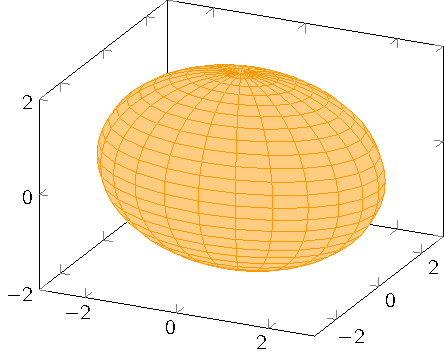
\includegraphics{./img/elde.pdf}
\end{minipage}

\begin{minipage}[c]{0.45\textwidth}
  {\bf Elipsoide imaginario}\vspace{1em}\\
  $\displaystyle -\frac{{x}^2}{a^2} - \frac{{y}^2}{b^2} - \frac{{z}^2}{c^2} = 1$
\end{minipage}\hfill
\begin{minipage}[]{0.45\textwidth}
\hfill
\end{minipage}

\begin{minipage}[c]{0.45\textwidth}
  {\bf Hiperboloide de una hoja}\vspace{1em}\\
  $\displaystyle \frac{{x}^2}{a^2} + \frac{{y}^2}{b^2}-\frac{{z}^2}{c^2} = 1$
\end{minipage}\hfill
\begin{minipage}[]{0.45\textwidth}
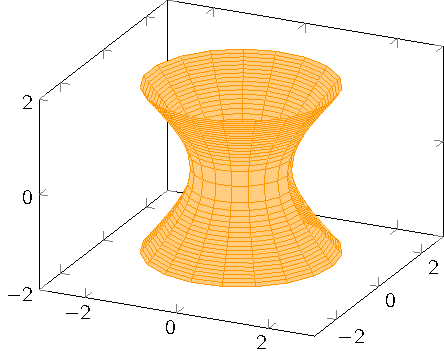
\includegraphics{./img/hip1.pdf}
\end{minipage}

\begin{minipage}[c]{0.45\textwidth}
  {\bf Hiperboloide de dos hojas}\vspace{1em}\\
  $\displaystyle \frac{{x}^2}{a^2} - \frac{{y}^2}{b^2}-\frac{{z}^2}{c^2} = 1$
\end{minipage}\hfill
\begin{minipage}[]{0.45\textwidth}
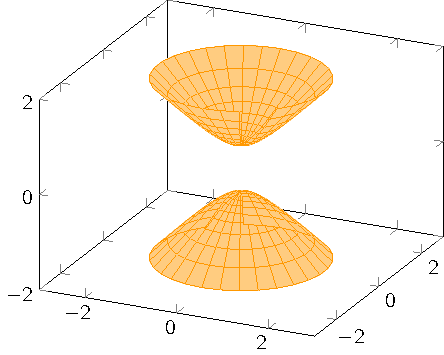
\includegraphics{./img/hip2.pdf}
\end{minipage}

\begin{minipage}[c]{0.45\textwidth}
  {\bf Cono}\vspace{1em}\\
  $\displaystyle \frac{{x}^2}{a^2} + \frac{{y}^2}{b^2}-\frac{{z}^2}{c^2} = 0$
\end{minipage}\hfill
\begin{minipage}[]{0.45\textwidth}
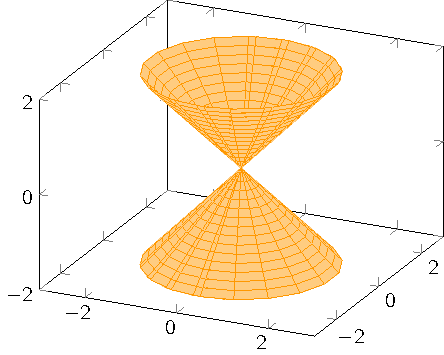
\includegraphics{./img/cono.pdf}
\end{minipage}

\begin{minipage}[c]{0.45\textwidth}
  {\bf Cono imaginario}\vspace{1em}\\
  $\displaystyle \frac{{x}^2}{a^2} + \frac{{y}^2}{b^2}+\frac{{z}^2}{c^2}=0$
\end{minipage}\hfill
\begin{minipage}[]{0.45\textwidth}
\hfill
\end{minipage}

\vspace{1em}

Rango de $\mathcal A = 2$.

Consideramos cuádricas con centro y rango $2$ en el sistema de referencia $\mathcal R$.

\vspace{1em}

\begin{minipage}[c]{0.45\textwidth}
  {\bf Cilindro elíptico}\vspace{1em}\\
  $\displaystyle \frac{{x}^2}{a^2} + \frac{{y}^2}{b^2}=1$
\end{minipage}\hfill
\begin{minipage}[]{0.45\textwidth}
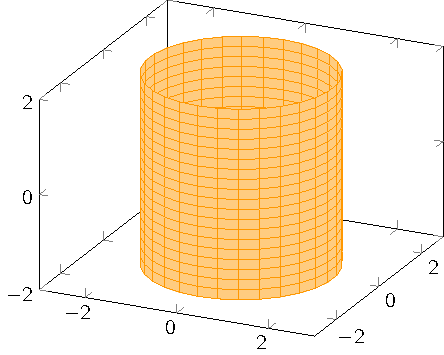
\includegraphics{./img/celi.pdf}
\end{minipage}

\begin{minipage}[c]{0.45\textwidth}
  {\bf Cilindro imaginario}\vspace{1em}\\
  $\displaystyle -\frac{{x}^2}{a^2} - \frac{{y}^2}{b^2}=1$
\end{minipage}\hfill
\begin{minipage}[]{0.45\textwidth}
\hfill
\end{minipage}

\begin{minipage}[c]{0.45\textwidth}
  {\bf Cilindro hiperbólico}\vspace{1em}\\
  $\displaystyle \frac{{x}^2}{a^2} - \frac{{y}^2}{b^2}=1$
\end{minipage}\hfill
\begin{minipage}[]{0.45\textwidth}
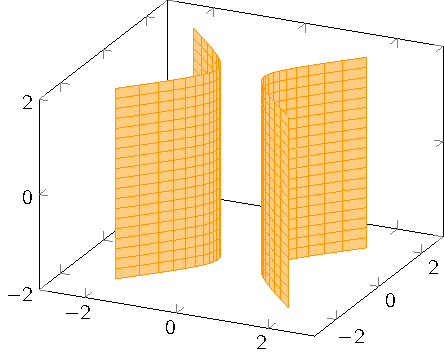
\includegraphics{./img/chip.pdf}
\end{minipage}

\begin{minipage}[c]{0.45\textwidth}
  {\bf Par de planos reales}\vspace{1em}\\
  $\displaystyle \frac{{x}^2}{a^2} - \frac{{y}^2}{b^2}=0$
\end{minipage}\hfill\vspace{1em}
\begin{minipage}[]{0.45\textwidth}
\hfill
\end{minipage}

\begin{minipage}[c]{0.45\textwidth}
  {\bf Par de planos imaginarios}\vspace{1em}\\
  $\displaystyle \frac{{x}^2}{a^2} + \frac{{y}^2}{b^2}=0$
\end{minipage}\hfill\vspace{1em}
\begin{minipage}[]{0.45\textwidth}
\hfill
\end{minipage}

\vspace{1em}

Rango de $\mathcal A = 1$.

Consideramos cuádricas con centro y rango $1$ en el sistema de referencia $\mathcal R$.

\vspace{1em}

\begin{minipage}[c]{0.45\textwidth}
  {\bf Par de planos paralelos}\vspace{1em}\\
  $\displaystyle \frac{{x}^2}{a^2}=1$
\end{minipage}\hfill\vspace{1em}
\begin{minipage}[]{0.45\textwidth}
\hfill
\end{minipage}

\begin{minipage}[c]{0.45\textwidth}
  {\bf Par de planos imaginarios paralelos}\vspace{1em}\\
  $\displaystyle \frac{{x}^2}{a^2} =-1$
\end{minipage}\hfill\vspace{1em}
\begin{minipage}[]{0.45\textwidth}
\hfill
\end{minipage}

\begin{minipage}[c]{0.45\textwidth}
  {\bf Plano doble}\vspace{1em}\\
  $\displaystyle {{x}^2} = 0$
\end{minipage}\hfill\vspace{1em}
\begin{minipage}[]{0.45\textwidth}
\hfill
\end{minipage}


\subsection{\bf  C\'onicas con centro en $\mathbb{R}^2$.}

\vspace{.5cm}

Dada una c\'onica $\cal C$ con centro consideramos el sistema de referencia
${\cal R}=\{A; e_1,e_2\}$ donde $A$
es el centro y $e_1,e_2$ es una base ortonormal de vectores propios de la matriz $\cal A$. Se tienen los siguientes casos

\begin{minipage}[c]{0.45\textwidth}
  {\bf Elipse}\vspace{1em}\\
  $\displaystyle \frac{{x}^2}{a^2} + \frac{{y}^2}{b^2} = 1$
\end{minipage}\hfill
\begin{minipage}[]{0.35\textwidth}
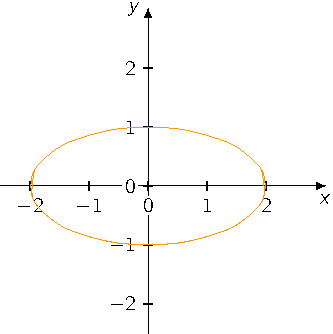
\includegraphics{./img/elip.pdf}
\end{minipage}

\begin{minipage}[c]{0.45\textwidth}
  {\bf Hipérbola}\vspace{1em}\\
  $\displaystyle \frac{{x}^2}{a^2} - \frac{{y}^2}{b^2} = 1$
\end{minipage}\hfill
\begin{minipage}[]{0.35\textwidth}
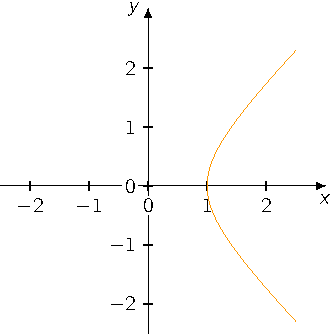
\includegraphics{./img/hipe.pdf}
\end{minipage}



\vspace{.8cm}

\begin{tabular}{ll}
{\it Elipse imaginaria}  &
$
-\frac{{x}^2}{a^2} - \frac{{y}^2}{b^2} = 1
$
\vspace{.4cm}
\\

{\bf  Par de rectas reales concurrentes}  &
$
\frac{{x}^2}{a^2} - \frac{{y}^2}{b^2}=0
$
\vspace{.4cm}
\\
{\it Par de rectas imaginarias} &
$
\frac{{x}^2}{a^2} + \frac{{y}^2}{b^2}=0
$
\vspace{.4cm}
\\
{\bf  Par de rectas reales paralelas}  &
$
\frac{{x}^2}{a^2}=1
$
\vspace{.4cm}
\\
{\it Par de rectas imaginarias paralelas}  &
$
-\frac{{x}^2}{a^2} = 1
$
\vspace{.4cm}
\\
{\bf  Recta doble}  &
$
{{x}^2} = 0
$
\vspace{.3cm}
\\
\end{tabular}
\subsubsection{\bf  Elementos notables de las c\'onicas y cu\'adricas con centro.}

\begin{ndef}[Centro]
	Es el centro de simetría de la cónica, es decir, el punto $A$ tal que la reflexión $\sigma_A$ mantiene invariante la cónica. Es importante notar que no todas las cónicas tienen centro.
\end{ndef}


\begin{ndef}[Ejes]
	 Son los ejes de simetr\'ia. Cada eje es una recta que pasa por el centro y tiene como vector director a un vector propio de la matriz $\cal A$. En $\mathbb{R}^2$ (respectivamente $\mathbb{R}^3$) se consideran dos (respectivamente tres)  ejes perpendiculares pasando por el centro.
\end{ndef}

\begin{ndef}[Vértices]
	La intersecci\'on de los ejes con la c\'onica o cu\'adrica.
\end{ndef}


\subsection{\bf Cu\'adricas sin centro en $\mathbb{R}^3$.}


Sea $\cal Q$ una cu\'adrica sin centro tal que el rango de $\cal A$ sea $2$. Entonces los valores propios son
$\lambda_1,\lambda_2 \neq 0$ y $\lambda_3=0$. Tomamos el sistema de referencia ${\cal R} = \{O; e_1,e_2,e_3\}$ con una base de vectores propios y la ecuaci\'on queda de la forma

\vspace{.3cm}

\[
{\cal Q} \, \, \equiv \, \, \lambda_1 x^2 + \lambda_2 y^2 + \beta_1 x + \beta_2 y + \beta_3 z + \gamma = 0
\]

\vspace{.2cm}

Consideramos un nuevo sistema de referencia $\overline{{\cal R}} = \{A;e_1,e_2,e_3\}$ de manera que el origen
$A=(\alpha_1,\alpha_2,\alpha_3)$ nos permita obtener cuadrados perfectos en $\overline{x}=x-\alpha_1$ e
$\overline{y}=y-\alpha_2$. La nueva ecuaci\'on es
\[
{\cal Q} \, \, \equiv \, \, \lambda_1 \overline{x}^2 + \lambda_2 \overline{y}^2 +
\overline{\beta}_3 \overline{z} = 0
\]
donde $\overline{\beta}_3\neq 0$ ya que la cu\'adrica no tiene centro. Esto nos permite obtener las ecuaciones reducidas para el caso sin centro.


\subsubsection{Ecuaciones reducidas para cuádricas sin centro.}

Rango $\cal A$ $=2$.

\begin{minipage}[c]{0.45\textwidth}
  {\bf Paraboloide elíptico}\vspace{1em}\\
  $\displaystyle z = \frac{x^2}{a^2} + \frac{y^2}{b^2}$
\end{minipage}\hfill
\begin{minipage}[]{0.45\textwidth}
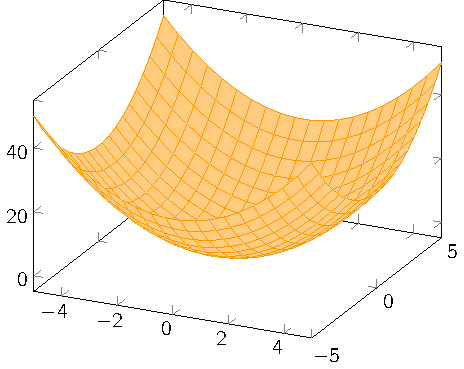
\includegraphics{./img/peli.pdf}
\end{minipage}

\begin{minipage}[c]{0.5\textwidth}
  {\bf Paraboloide hiperbólico}\vspace{1em}\\
  $\displaystyle z = \frac{x^2}{a^2} - \frac{y^2}{b^2}$
\end{minipage}\hfill
\begin{minipage}[]{0.5\textwidth}
    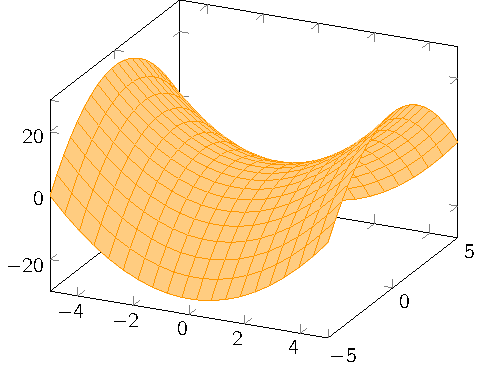
\includegraphics{./img/phip.pdf}
\end{minipage}

Rango $\cal A$ $=1$.

\begin{minipage}[c]{0.45\textwidth}
  {\bf Cilindro parabólico}\vspace{1em}\\
  $\displaystyle z = \frac{x^2}{a^2}$
\end{minipage}\hfill
\begin{minipage}[]{0.45\textwidth}
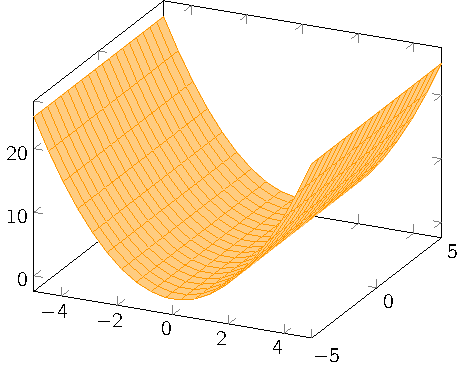
\includegraphics{./img/cpar.pdf}
\end{minipage}


\subsection{Cónicas sin centro en $\mathbb{R}^2$.}


\begin{minipage}[c]{0.45\textwidth}
  {\bf Parábola}\vspace{1em}\\
  $\displaystyle y = \frac{x^2}{a^2}$
\end{minipage}\hfill
\begin{minipage}[]{0.35\textwidth}
  \begin{tikzpicture}
\sffamily
  \tkzInit[ymin=-2.5,ymax=2.5,xmin=-2.5,xmax=2.5]
  \tkzAxeXY
  \draw[scale=1,domain=-1.7:1.7,smooth,variable=\x,500, samples=20] plot ({\x},{\x*\x});
\end{tikzpicture}
\end{minipage}



\subsection{Cuádricas sin centro}

\newpage

\section{El plano proyectivo}

Para definir correctamente el plano proyectivo, primero realizaremos una "definición"\ a través de un caso concreto. Situémonos en $\mathbb{R}^3$. Ahora definamos el plano $\pi \equiv z = 1 \equiv$ plano afín, así como el plano $\pi_0 \equiv z = 0 \equiv$ plano vectorial, y el punto $O = (0,0,0)$ el origen.


Entonces definimos el plano proyectivo $\mathbb{P}^2$ como el conjunto formado por las intersecciones de cada recta vectorial de $\mathbb{R}^3$ con el plano $\pi$. Este conjunto contiene a todos los puntos del plano $\pi$(dado un punto del plano siempre puedes encontrar una recta centrada en el origen que pase por el), pero ademas, contiene la intersección de las rectas vectoriales paralelas a dicho plano. Por ello llamaremos "puntos" del plano proyectivo a cada intersección de una recta vectorial con $\pi$ y en concreto "puntos en el infinito"\ aquellos puntos generados por una recta paralela a $\pi$. Simbólicamente:
$$\mathbb{P}^2 = \mathbb{R}^2\ \cup \{\text{puntos del infinito}\}$$
Ahora definimos la rectas de $\mathbb{P}^2$ como la intersección de un plano vectorial con $\pi$, de manera que de la misma que forma que ocurría con los puntos, $\mathbb{P}^2$ contiene a todas las rectas de $\mathbb{R}^2$ y a un recta más, que es la definida por el plano $\pi_0 \equiv z= 0$ a la que llamaremos recta del infinito ($r_\infty$). Si nos fijamos, esta recta contiene a todos los puntos del infinito, por tanto:
$$\mathbb{P}^2 = \mathbb{R}^2\ \cup r_\infty$$

\begin{nth}
Sean P y Q dos puntos distintos de $\mathbb{P}^2$, existe una única recta proyectiva que contiene a P y Q. A esta la llamaremos $P \vee Q$
\end{nth}
\begin{proof}

De lo estudiado en espacio afín sabemos que dos rectas vectoriales distintas determinan un plano vectorial único que las contiene, por tanto, utilizando la biyección que conocemos entre rectas vectoriales y puntos de $\mathbb{P}^2$ y planos vectoriales y rectas de $\mathbb{P}^2$, la prueba del resultado es trivial.
\end{proof}

\begin{nth}
Dos rectas proyectivas se cortan en único  punto proyectivo
\end{nth}
\begin{proof}
La demostración es similar a la del teorema anterior usando que dos planos vectoriales distintos se cortan un una única recta vectorial
\end{proof}

\textbf{Consecuencias:}

Una recta $r$ en $\mathbb{R}^2$ identifica a una única recta en $\mathbb{P}^2$ que contiene a:
\begin{nlist}

	\item $r \cap \mathbb{R}^2 =$ la recta de siempre.
%%%TODO Pensar una forma de escribirlo mejor
	\item $r \cap \{$\textit{puntos\ en\ el\ infinito}\} = $r \cap r_\infty = 1$ punto en el infinito.

\end{nlist}

Ahora, una vez comprendida la aproximación inicial necesaria para poder imaginarnos y comprender el plano proyectivo, veamos que se puede construir con dos planos cualesquiera con una serie de condiciones.


Sean dos planos $\pi'$ y $\pi_0'$, cumpliendo que:
\begin{nlist}
	\item $O \notin \pi'$
	\item $O \in \pi_0$
	\item $\pi\ ||\ \pi_0$
\end{nlist}
Con estos dos planos podemos realizar la misma construcción que realizamos al comienzo del tema y formando de nuevo el plano proyectivo $\mathbb{P}^2$.

Si nos fijamos, podemos decir que el plano proyectivo formado por cada par de planos es el mismo porque los elementos de ambos están determinados inequívocamente por las rectas vectoriales y los planos vectoriales, por tanto, ambos son iguales, con la diferencia de que la llamada "recta en el infinito" es distinta, que estaría determinada respectivamente por los planos $\pi_0$ y $\pi_0'$

\begin{nprop}
Sea $r \in \mathbb{P}^2 \implies \mathbb{P}^2 - r =$ plano afín.
\end{nprop}
%%%TODO Esto hace falta demostrarlo? En dicho caso, como se haría?

\begin{ndef}
Tres puntos no alineados $A,B,C \in \mathbb{P}^2$ definen único triángulo $ABC$, cuyos elementos son similares a los definidos para los triángulos en el plano afín
\end{ndef}

\begin{ndef}
Cuatro puntos no alineados 3 a 3 $A,B,C,D \in \mathbb{P}^2$ definen un único cuadrilátero, para el que definiremos los siguientes elementos:
\begin{itemize}
	\item Vértices: $A, B, C, D$
	\item Lados: $A\vee B, B\vee C, C\vee D, D\vee A$
	\item Puntos diagonales: $P = (B\vee C) \cap (D\vee A)$, $Q = (A\vee B) \cap (C\vee D)$
	\item Rectas diagonales: $A\vee C, B\vee D$
\end{itemize}
\end{ndef}

\begin{nth}[Teorema de Fano]
	Dada un cuadrilátero $ABCD \in \mathbb{P}^2$, los dos puntos diagonales $P$ y $Q$ y el punto de corte R de las dos rectas diagonales $R = (A \vee C)\cap (B\vee D)$, no están alineados
\\


\end{nth}
\begin{proof}
	Para llevar a cabo esta demostración trabajaremos en el plano afín $\mathbb{P}^2 -r$, con $r = P\vee Q$. De esta manera obtenemos que el cuadrilátero $ABCD$ que obtenemos en dicho plano afín es un paralelogramo (pues sus lados son paralelos por estar sus puntos de corte en el infinito).

	Por tanto, como sabemos del estudio del plano afín que las diagonales de un paralelogramos se cortan en su punto medio, $R$. Consecuentemente, $P$ y $Q$ pertenecen a $r$ y R al plano afín $\mathbb{P}^2 - r \implies R \notin r$ luego $P,Q$ y $R$ no están alineados.
	\end{proof}

\begin{nprop}
	Si $r$, $s$ son dos rectas en $\mathbb P^2$ con $r\ne s$, entonces:
	\[
	r \cap s = 1 \text { punto } \begin{cases}
	\in \R^2 \equiv \text{ no son paralelas}\\

	\in r_\infty \equiv \text{ son paralelas}

\end{cases}
	\]
\end{nprop}

\begin{nth}[Teorema de Desargues]
	Sean $ABC$, $A'B'C'$ dos triángulos en $\mathbb P^2$ cuyos vértices homólogos son diferentes y los lados homólogos también tales que los lados homólogos se cortan en tres puntos alineados.\\
	Entonces, las rectas que unen los vértices homólogos son concurrentes
\end{nth}

Tenemos también versiones afines del teorema de Desargues:

\begin{nth}[Versión afín del Teorema de Desargues]
	Sean dos triángulos en el afín tales que los lados homólogos no son paralelos y se cortan en tres puntos alineados.\\
	  Entonces las rectas que unen los vértices homólogos son o bien concurrentes o bien paralelas
\end{nth}

\begin{nth}[Versión equivalente 2]
	Sean $ABC$,$A'B'C'$ dos triángulos en el afín tales que los pares de lados homólogos son paralelos.\\
	Entonces, las rectas que unen los vértices homólogos son concurrentes o son paralelas.
\end{nth}


%%%TODO: Definir Q.
\begin{nth}[Versión equivalente 3]
	En el afín $\mathbb P^2 - P\vee Q$ con $P$ el punto de corte de las rectas que unen los vértices homólogos y $Q$  el punto de corte, si un paralelogramo está inscrito en un cuadrilátero.\\
	Entonces, la otra diagonal del cuadrilátero es paralela al otro par de lados del paralelogramo.
\end{nth}

\begin{nota}
	Los enunciados afines son equivalentes al enunciado proyectivo. Por tanto, probando una de las versiones habremos probado todas.
\end{nota}
\begin{proof}
	Vamos a probar la versión afín 2.\\
	Los lados homólogos de los triángulos $ABC$, $A'B'C'$ de $\R^2$ son paralelos. Entonces, existe una dilatación:
	\[
	f: \R^2 \to \R^2 \begin{cases}
	A \mapsto A'\\
	B \mapsto B'\\
	C \mapsto C'

\end{cases}
	\]
	Que lleva uno en otro.
	\begin{enumerate}
	\item Si $f$ es una traslación, $f = t_v$, entonces $\vec{AA'}= \vec{BB'} = \vec{CC'}=v$
	\item Si $f$ es una homotecia, $f= h_{p,\lambda}$, con $\lambda \ne 0, 1$, entonces $(P,A,A')$, $(P,B,B')$, $(P,C,C')$ están alineados y $A\vee A'$, $B \vee B'$ y $C \vee C'$ concurren.
\end{enumerate}
\end{proof}

\begin{ndef}[Hexágono]
    Si dados 6 puntos, $A,B,C,D,E,F$ los consecutivos no están alineados 3 a 3, entonces forman el hexágono $ABCDEF$.
\end{ndef}

\begin{nth}[Teorema de Pappus]\hfill\\
\begin{minipage}[c]{0.4\textwidth}
Si los vértices de un hexágono en $\mathbb P^2$ están alternativamente sobre 2 rectas distintas, entonces los 3 pares de lados opuestos se cortan en 3 puntos alineados.
\end{minipage}\hfill
\begin{minipage}[]{0.6\textwidth}
       \begin{tikzpicture}[scale=1.5]
  \sffamily
  \tkzSetUpPoint[size=10,color=900, fill=700]
  % Definimos los vértices
  \tkzDefPoint(0,0){O}
  \tkzDefPoint(5,3){P}
  \tkzDefPoint(5,0){P'}

  %\tkzDefMidPoint(A,B) \tkzGetPoint{P}

  \tkzDefPointWith[linear, K=0.3](O,P) \tkzGetPoint{6}
  \tkzDefPointWith[linear, K=0.5](O,P) \tkzGetPoint{4}
  \tkzDefPointWith[linear, K=0.8](O,P) \tkzGetPoint{2}
  \tkzDefPointWith[linear, K=0.3](O,P') \tkzGetPoint{5}
  \tkzDefPointWith[linear, K=0.5](O,P') \tkzGetPoint{1}
  \tkzDefPointWith[linear, K=0.8](O,P') \tkzGetPoint{3}

  \tkzDrawSegment[color=500](O,P)
  \tkzDrawSegment[color=500](O,P')

  \tkzDrawSegments[color=700](6,1 1,2 3,4 4,5 6,3 5,2)

  \tkzDrawPoints(6,4,2)
  \tkzLabelPoints[above=0.5em](6,4,2)

  \tkzDrawPoints(5,1,3)
  \tkzLabelPoints[below=0.5em](5,1,3)

  \tkzInterLL(5,4)(6,1) \tkzGetPoint{A}
  \tkzInterLL(5,2)(6,3) \tkzGetPoint{B}
  \tkzInterLL(4,3)(1,2) \tkzGetPoint{C}

  \tkzDefPointWith[linear, K=2.5](A,C) \tkzGetPoint{C'}
  \tkzDefPointWith[linear, K=-2](A,C) \tkzGetPoint{A'}

  \tkzDrawSegment[color=300](A',C')

  \tkzLabelSegment[below=0.5em, pos=.1](A',C'){$r$}

  \tkzDrawPoints(B, C)
  \tkzLabelPoints[right=0.5em](B, C)

  \tkzDrawPoints(A)
  \tkzLabelPoints[left=0.5em](A)

  %\tkzText(1,1){$\alpha$}
  %\tkzText(2,1){$\alpha$}

\end{tikzpicture}
\end{minipage}

\end{nth}


\begin{nth}[Versión afín del teorema de Pappus]\hfill\\
\begin{minipage}[c]{0.45\textwidth}
  Dado un hexágono en el plano afín cuyos vértices están alternativamente en dos rectas distintas $s$ y $s'$. Si los pares de lados opuestos son paralelos, entonces el tercer par de lados opuestos también es paralelo.
\end{minipage}\hfill
\begin{minipage}[]{0.55\textwidth}
       \begin{tikzpicture}[scale=1.5]
  \sffamily
  \tkzSetUpPoint[size=10,color=900, fill=700]
  % Definimos los vértices
  \tkzDefPoint(0,0){O}
  \tkzDefPoint(5,3){P}
  \tkzDefPoint(5,0){P'}

  %\tkzDefMidPoint(A,B) \tkzGetPoint{P}

  \tkzDefPointWith[linear, K=0.3](O,P) \tkzGetPoint{6}
  \tkzDefPointWith[linear, K=0.5](O,P) \tkzGetPoint{4}
  \tkzDefPointWith[linear, K=0.8](O,P) \tkzGetPoint{2}
  \tkzDefPointWith[linear, K=0.3](O,P') \tkzGetPoint{5}
  \tkzDefPointWith[linear, K=0.5](O,P') \tkzGetPoint{1}
  \tkzDefPointWith[linear, K=0.8](O,P') \tkzGetPoint{3}

  %\tkzDrawSector[color=300, fill=50](P,C')(A')
  %\tkzDrawSector[color=300, fill=50](P,D')(B')

  \tkzDrawSegment[color=500](O,P)
  \tkzDrawSegment[color=500](O,P')

  \tkzDrawSegments[color=700](5,6 6,1 1,2 2,3 3,4 4,5)

  \tkzDrawPoints(6,4,2)
  \tkzLabelPoints[above=0.5em](6,4,2)

  \tkzDrawPoints(5,1,3)
  \tkzLabelPoints[below=0.5em](5,1,3)

  \tkzMarkSegments[mark=|,color=900](5,6 2,3)
  \tkzMarkSegments[mark=||,color=900](5,4 1,2)
  \tkzMarkSegments[mark=|||,color=900](1,6 3,4)

  %\tkzText(1,1){$\alpha$}
  %\tkzText(2,1){$\alpha$}

\end{tikzpicture}
\end{minipage}

\end{nth}

%%% TODO: Completar demostración
%%% TODO: Si se quiere, cambiar el dibujo para que los nombres sean 1,2,3,4,5,6 y se facilite la notación
\begin{proof}[Demostración de la versión afín]\hfill


\begin{nlist}
	\item Si $s \parallel s'$ %%% TODO: Completar demostración e incluir dibujo para paralelas y no paralelas
	\item Si $s\cap s' = P$. Tenemos que probar que:
	$$\begin{rcases}
	P_1\vee P_2 \parallel P_4 \vee P_5\\
	P_2\vee P_3 \parallel P_5 \vee P_6
\end{rcases}\implies P_3 \vee P_4 \parallel P_6 \vee P_1 $$

\textit{Caso primer hexágono}:\\ %incluir dibujo primer hexagono
Por el Teorema de Thales sabemos que $\frac{PP_5}{PP_1}=\frac{PP_4}{PP_2}$ y que $\frac{PP_3}{PP_5}=\frac{PP_2}{PP_6}$. Si multiplicamos ambas igualdades nos queda que $\frac{PP_3}{PP_1} = \frac{PP_4}{PP_6}$, por lo que aplicando una última vez el Teorema de Thales nos queda que $P_1 P_6$ es paralelo a $P_3 P_4$.

\textit{Caso segundo hexágono}:\\
Teniendo este caso, cogemos los dos triángulos enfrentados por los vértices $P_1P_2P$ y $P_4P_5P$.  Sabemos %por la magia de aros TODO:Demostrar
que $\frac{PP_4}{PP_2} = \frac{PP_5}{PP_1} \iff P_1\vee P_2 || P_4\vee P_3$. Por ello, una vez sabemos aplicar esta propiedad, la demostración es análoga a la anterior.
\end{nlist}
\end{proof}


%TODO:Dejado como ejercicio
%TODO:incluir dibujo

\begin{ndef}[Punto Diagonal]
	Un punto diagonal es el punto donde dos lados opuestos de una cuadrilátero se cortan. Cada cuadrilátero tiene dos puntos diagonales.
\end{ndef}

\begin{nth}
    Si un cuadrilátero $A'B'C'D'$ está inscrito en otro $ABCD$ de forma que las cuatro diagonales son concurrentes, entonces los cuatro puntos diagonales (dos de cada cuadrilátero) están alineados.
\end{nth}

\begin{proof}
	Para demostrarlo, haremos un teorema equivalente en el afín, quitando una recta que no moleste.
\end{proof}

%TODO: formalizar
	$P \in \mathbb{P}^2 \equiv$ recta vectorial de$ \mathbb{R}^3 \equiv (x_0,x_1,x_2) $
	Entonces, Para algún $x_i \ne 0$, listas proporcionales representan el mismo V y representan el mismo P.

\begin{ndef}[Coordenadas homogéneas]
Dado un punto en el espacio proyectivo, llamamos coordenadas homogéneas de dicho punto a cada terna $(x_0,x_1,x_2)$, tal que, vista como un punto de $\mathbb{R}^3$, pertenece a la recta vectorial de $\mathbb{R}^3$ que lo define.
\end{ndef}

Es conveniente indicar que ternas proporcionales representan el mismo punto de $\mathbb{P}^2$ pues los puntos de $\mathbb{R}^3$ con coordenadas proporcionales pertenecen a la misma recta vectorial.

Ahora bien, tengamos un punto en $\mathbb{R}^2$ de coordenadas $(x,y)$, que sabemos que esta asociado a un único punto de $\mathbb{P}^2$. Definimos las coordenadas homogéneas asociadas a dicho punto como $(x,y,1)$ y todo el resto de coordenadas equivalentes. Del mismo modo si tenemos un punto en el proyectivo  $(x_0, x_1, x_2)$ este equivale con $(x_0/x_2, x_1/x_2)$.

Si observamos la primera parte siempre se puede hacer. La segunda sin embargo no, porque si no sería una correspondencia biyectiva, la cual sabemos que no existe. Cuando $x_2 = 0$ estaremos trabajando con puntos del infinito, los cuales ya sabemos que no existen en el afín.\\

Sean $A$ y $B$ dos puntos distintos en el afín con $A =(1,2)$ y $B=(-1,1)$ sabemos que definen la recta $A \vee B = \{ \lambda (1,2) + \mu (-1,1) \backslash \lambda + \mu = 1\}$.\\
Ahora bien, en $\mathbb{P}^2$, teniendo dos puntos $A(a_1,a_2,a_3), B(b_1,b_2,b_3)$, que sabemos que definen rectas vectoriales en $\mathbb{R}^3$, y por tanto generan un plano vectorial, el cual puede verse como una recta proyectiva. Entonces $A\vee B = \{ \lambda (a_1,a_2,a_3) + \mu (b_1,b_2,b_3)\backslash \lambda, \mu \ne 0 \} = \{  \{ (a_1,a_2,a_3) + \alpha (b_1,b_2,b_3)\backslash \alpha  \in \mathbb{R}\} \cup  \{(b_1,b_2,b_3) \}$

\begin{ndef}[Ecuación de una recta en el plano afín.]
Dada una recta perteneciente al plano afín, sabemos que se puede escribir de la forma $r = \{(x,y) \in \mathbb{R}^2\ \backslash\ ax + by + c = 0, a \textup{ ó } b \neq 0\}$. Entonces llamamos ecuación de r a la expresión $ax + by + c = 0$
\end{ndef}
Sabemos que dos rectas son iguales si y solo sus ecuaciones son proporcionales

\begin{ndef}[Ecuación de una recta en el plano proyectivo.]
Dada una recta perteneciente al plano proyectivo, sabemos que se puede escribir de la forma $r = \{(x_0,x_1,x_2) \in \mathbb{P}^2\ \backslash\ a_0x_0+a_1x_1+a_2x_2 = 0\}$ con algun $a_i \neq 0$ (r esta definido por un plano vectorial que sabemos que se puede escribir de esa forma). Entonces llamamos ecuación de r a la expresión $a_0x_0+a_1x_1+a_2x_2 = 0$
\end{ndef}
Sabemos que dos planos son iguales si y solo si sus ecuaciones son proporcionales, por lo tanto dos rectas en el proyectivo lo serán también si y solo si sus ecuaciones son proporcionales

Por  último nos quedaría considerar la correspondencia entre la recta proyectiva y la afín, el cual realizaremos de modo análogo. Esto implicará los pasos punto a punto, y, quitando los puntos de infinito. La recta del infinito obviamente no se pasará

\begin{nth}
	Sean $ABCD$ y $A'B'C'D'$ dos cuadriláteros en el plano protectivo $\mathbb{P}^2$ tales que $A'B'C'D'$ está inscrito en $ABCD$ y sus cuatro rectas diagonales son concurrentes. Entonces  los cuatro puntos diagonales de los cuadrilateros están alineados.
\end{nth}

\begin{proof} \hfill
	\begin{nlist}
	\item Versión afín del teorema: $ABCD$ y $A'B'C'D'$ dos cuadriláteros en $\mathbb{R}^2$ tales que $A'B'C'D'$ está inscrito en $ABCD$, y sus cuatro rectas diagonales son concurrentes. Entonces, si $ABCD$ es un paralelograma, $A'B'C'D'$ también lo es.
	\item Probamos el teorema en el afín. Sea $\sigma$ la reflexión central de centro $O$, el punto donde se cortan las diagonales. Por ser $ABCD$ un paralelogramo, sabemos que $O$ es el punto medio de los vértices opuestos, luego:
	\[
	\begin{rcases}
		A \leftrightarrow^\sigma C\\
		B \leftrightarrow^\sigma D
\end{rcases} \implies
	\begin{rcases}
		A\vee B \leftrightarrow C \vee D\\
		A \vee D \leftrightarrow B \vee C
\end{rcases}
\]
Ahora, como por hipótesis sabemos que la recta $E \vee G$ pasa por $O$, entonces la reflexión central lleva la recta en ella misma, luego:
$$E = (A \vee B) \cap (E \vee G) \leftrightarrow^\sigma (C \vee D) \cap (E \vee G) = G$$
$$H = (A \vee D) \cap (F \vee H) \leftrightarrow^\sigma (B \vee C) \cap (F \vee H) = H$$
Ahora sabemos que una homotecia aplicada sobre una recta nos da una recta paralela a ella, y por tanto:
\[
\begin{rcases}
	E\vee H \leftrightarrow^\sigma F \vee G \implies E \vee G \parallel F \vee G\\
	E\vee F \leftrightarrow^\sigma E \vee F \implies E \vee F \parallel H \vee G
\end{rcases} \implies EFGH \text{ es un paralelogramo}
\]
\end{nlist}
\end{proof}

\begin{nth}
Sean, en $\mathbb P^2$ dos puntos $A$ y $B$ y 3 pares de rectas distintas tales que una pasa por $A$ y la otra por $B$. Se forman 3 cuadriláteros con vértices opuestos $A$ y $B$ y una recta diagonal $A\vee B$. Entonces, las otras 3 rectas diagonales son concurrentes
\end{nth}

%%%TODO Incluir dibujito
\begin{proof} \hfill
	\begin{nlist}
	\item Versión afín del teorema: En este caso, uno de los cuadriláteros será un paralelogramo y tendremos que, entonces. las 3 rectas diagonales $(\ne A\vee B)$ son concurrentes o paralelas
	\item Probamos ahora la versión afín.\\
	Supuesto que el par de rectas sobrantes no son paralelas:\\
	Consideramos los triangulos $CDE$ y $FGH$ mostrados en la figura. Entonces, sabemos que si dos triangulos poseen lados homólogos paralelos, son semejantes y existe una homotecia que lleva vertices en vertices homólogos, lo que demostría el teorema.
	%%% Esto último está demostrado?
	Ahora bien, por hipótesis sabemos que:
	$$C \vee D \parallel F \vee H$$
	$$C \vee E \parallel G \vee F$$
	Luego solo faltaría demostrar que $D \vee E \parallel G \vee H$. Ahora bien aplicando thales sobre el par de rectas no necesariamente paralelas:
	\[
	\begin{rcases}
		\frac{a+b}{a} = \frac{d+e+f}{d+e}\\
		\frac{a+b+c}{a+b} = \frac{d+e}{d}
\end{rcases} \implies \frac{(a+b+c)*(a+b)}{(a+b)*a} = \frac{(d+e+f)*(d+e)}{(d+e)*d} \implies
\]
$$\implies \frac{a+b+c}{a} = \frac{d+e+f}{d} \implies D \vee E \parallel G \vee H$$
Supuesto que el par de rectas sobrantes son paralelas:
%%% TODO Demostrar
\end{nlist}
\end{proof}

\subsection{Dualidad}

\begin{ndef}[Coordenadas homogéneas de la recta]
	Si $r \in \mathbb P ^2$ es una recta cuya ecuación es:
	\[
	a_0x_0 + a_1x_1 + a_2 x_2 = 0
	\]
	entonces, se llaman coordenadas homogéneas de la recta a la terna:
	\[
	(a_0,a_1,a_2)
	\]
\end{ndef}

Sea $r \in \mathbb P ^2$ una recta con $r$ con coordenadas homogéneas $(a_0,a_1,a_2)$  con algún $a_i \ne 0$. Entonces cualquier terna proporcional a esta representa la misma recta en $\mathbb{P}^2$, pues la ecuacion sería equivalente.

\begin{ndef}[Plano proyectivo dual]
	Se define el plano proyectivo dual como aquel que tiene como conjunto de puntos el conjunto de rectas de $\mathbb{P}^2$. Es decir :
	$$\mathbb{P}^{2*} = \{ (a_0,a_1,a_2) \ \text{ con algún $a_i\ne 0$}\}$$
\end{ndef}

\begin{ndef}[Plano proyectivo dual]
	El plano proyectivo dual es el conjunto de rectas de $\mathbb P ^2 \equiv \mathbb P^{2*}$ definido como:
	\[
	\mathbb P^{2*} = \{ (a_0,a_1,a_2) \ \text{ con algún $a_i\ne 0$}\}
	\]
\end{ndef}
De esta forma, tenemos dos copias del plano proyectivo, los $(a_0,a_1,a_2)\in \mathbb P^{2*}$ y los $\begin{pmatrix}
 x_0\\
 x_1\\
 x_2
\end{pmatrix}  \in \mathbb P ^2$. Con esto tenemos que:
\[
a_0 x_0 + a_1x_1 + a_2x_2 = \begin{cases}
	=0 \ \ \ \ P \in r\\
	\ne 0 \ \ \ \ P \notin r
\end{cases}
\]

\begin{ndef}[Recta del plano proyectivo dual]
	Una recta del plano proyectivo dual $\mathbb P^{2*}$ viene dada de la forma:
	\[
	\Lambda = \{ (a_0, a_1,a_2) \in \mathbb P^{2*} : \alpha_0a_0 + \alpha_1 a_1 + \alpha_2 a_2 = 0\}
	\]
	\[
	= \{ r \text{ recta de } \mathbb P ^2  : r \text { pasa por } P\} \ \ \ \text{ con } P = \begin{pmatrix}
 \alpha_0\\
 \alpha_1\\
 \alpha_2
\end{pmatrix}
	\]
	También son llamados haces de rectas de $\mathbb P^2$ que pasan por $P$.
\end{ndef}

\begin{nth}
	Existe un isomorfismo NATURAL entre $\mathbb P^2 $y $(\mathbb P^{2*})^*$
\end{nth}
\begin{nota}
	Lo que hace es volver a transformar los haces de rectas en puntos.
\end{nota}

\begin{nprop}[Propiedades]
	\begin{nlist}
	\item Una sucesión de puntos alineados en $\mathbb P^2$ son rectas concurrentes en $\mathbb P^{2*}$
\end{nlist}
\end{nprop}

\begin{nth}
	Por dos puntos distintos pasa una recta y solo una.
\end{nth}

\begin{nth}[Enunciado dual]
	Entre dos rectas del plano proyectivo existe un único punto de intersección entre ellas.
\end{nth}

\begin{ejemplo}
	Un triángulo
\end{ejemplo}
\begin{ndef}[Triángulo dual]
	Tres rectas no concurrentes(los vértices del original) y tres puntos de corte(las rectas del original)
\end{ndef}

\subsection{Proyectividades}

\begin{ndef}[Proyectividad]
	Una proyectividad es una aplicación:
	\[
	f: \mathbb P ^2 \to \mathbb P^2
	\]
	\[
	 \begin{pmatrix}
 x_0\\
 x_1\\
 x_2
\end{pmatrix}  \mapsto A  \begin{pmatrix}
 x_0\\
 x_1\\
 x_2
\end{pmatrix}  \
	\]
	Con $A$ una matriz $3\times 3$ regular. Esto define una aplicación:
	\[
	\bar{f} : \R^3 \to \R^3
	\]

\end{ndef}

\begin{nprop}[Propiedades de $\bar{f}$]\hfill
	\begin{nlist}
	\item $\bar{f}$ lleva rectas vectoriales en rectas vectoriales
	\item $\bar{f}$ lleva planos vectoriales en planos vectoriales
	\item $\bar{f}$ lleva vectores linealmente independientes en vectores linealmente independientes.
	\item Ídem con vectores linealmente dependientes.
\end{nlist}
\end{nprop}

\begin{nprop}[Propiedades de $f$]\hfill
	\begin{nlist}
	\item $f$ lleva puntos de $\mathbb P^2$ en puntos de $\mathbb P^2$
	\item $f$ lleva rectas de $\mathbb P^2$ en rectas de $\mathbb P^2$
	\item $f$ lleva puntos no alineados a puntos no alineados
	\item Ídem con puntos sí alineados
\end{nlist}
\end{nprop}

\begin{nprop}
	Si $A$ es la matriz de una proyectividad y $\lambda \ne 0$, entonces $\lambda A$ y $A$ inducen la misma proyectividad.
\end{nprop}

\begin{nprop}
	Si tenemos una proyectividad $f$ con matriz $A$ y otra $g$ con una matriz $B$, la composición de ambas es otra proyectividad $go f$ con matriz $BA$
\end{nprop}

\begin{nprop}
	Si $f$ es una proyectividad de matriz $A$ y $A$ tiene inversa, entonces $f$ es biyectiva
\end{nprop}

\begin{nth}
	Toda proyectividad tiene al menos un punto fijo
\end{nth}
\begin{proof}\hfill\\
Es análoga a la del teorema: Todo isomorfismo lineal de $\R^3$ tiene al menos un vector propio.
\end{proof}
\subsubsection{Relación entre afinidades y proyectividades}

Si $h: \R^2 \to \R^2$ es una afinidad de la forma:
\[
h \begin{pmatrix}
x\\
y
\end{pmatrix}  = \begin{pmatrix}
 \alpha & \beta \\
 \gamma & \delta
\end{pmatrix} \begin{pmatrix}
x\\
y
\end{pmatrix} + \begin{pmatrix}
b_1\\
b_2
\end{pmatrix}
\]
podemos definir una proyectividad $\bar h : \mathbb P ^2 \to \mathbb P^2$ tal que:
\[
\bar{h} \begin{pmatrix}
 x_0\\
 x_1\\
 x_2
\end{pmatrix}  = \begin{pmatrix}
 1 & 0 & 0 \\
 b_1 & \alpha & \beta \\
 b_2 & \gamma & \delta
\end{pmatrix} \begin{pmatrix}
 x_0\\
 x_1\\
 x_2
\end{pmatrix}
\]

\begin{nprop}
	Toda afinidad se extiende a una proyectividad. En ella, se fija $r_\infty$.
\end{nprop}

\begin{nprop}
	$\bar h$ actúa sobre $r_\infty$, la lleva sobre sí misma.
\end{nprop}
%%% TODO: Añadir ejemplos de proyectividades

\begin{nth}
	Si $f: \mathbb P^2 \to \mathbb P^2$ es una proyectividad, entonces:
	\[
	\text{ $f$ viene de una afinidad } \iff f(r_\infty) = r_\infty
	\]
\end{nth}
\begin{proof}
	Sea $A$ la matriz:
	\[
	\begin{pmatrix}
 a_0& b_0 & c_0 \\
 a_1 & b_1 & c_1\\
 a_2 & b_2 & c_2
\end{pmatrix}
	\]
	Tenemos que tener que $f\begin{pmatrix}
0\\
1\\
0
\end{pmatrix} \mapsto \begin{pmatrix}
b_0\\
\\

\end{pmatrix} \implies b_0 = 0 $. Idem con $\begin{pmatrix}
0\\
0\\
1
\end{pmatrix} \implies c_0 = 0 $ y tenemos que tener que $a_0 \ne 0$. Por tanto, la matriz será de la forma:
\[
\dfrac{1}{a_0} A = \begin{pmatrix}
 1& 0 & 0 \\
  &  & \\
  & &
\end{pmatrix}
\]
(Los huecos en blanco no son relevantes). De esta forma, tenemos que está definida a partir de una afinidad.
\end{proof}

\begin{ncor}
	Si $f: \mathbb P^2 \to \mathbb P^2$ es una proyectividad. $r\subset \mathbb P^2$ es una recta con $f(r) = r$.
	Entonces, sobre el afín $\mathbb P^2 -r$, $f|_{\mathbb P^2 -r}$ es una afinidad.
\end{ncor}

\subsection{Proyectividades y dualidad}

\begin{nth}
	Toda proyectividad de $\mathbb P^2$ tiene al menos un punto fijo.
\end{nth}

\begin{nth}[Dual]
	Toda proyectividad de $\mathbb P^2$ tiene al menos una recta fija
\end{nth}
\begin{proof}
	Por el teorema anterior, la demostración queda hecha. Ya que tener la demostración en el proyectivo nos la da en el proyectivo dual.
\end{proof}


\begin{nota}
	Sea $\phi: V^n \to V^n $ lineal con $\phi(v) = \lambda v$. Sean $\lambda_1,\cdots,\lambda_k$ valores propios. Entonces, si $f:\mathbb P^2 \to \mathbb P^2$ es una proyectividad, los valores propios de $\phi$ son los puntos fijos de $f$.
\end{nota}

\begin{nota}
	Si $V_1,\cdots,V_k$ son los subespacios de los vectores propios de $\phi$, estos están contenidos en $V:(e_{11},\cdots,e_{n1}), \cdots, (e_{1k},\cdots,e_{nk})$ una base de cada uno de los $V_\lambda$, entonces:
	\[
	dim(V_{\lambda_1}) + \cdots + dim(V_{\lambda_k}) = dim(V)
	\]
	y los vectores anteriores son l.i. de $V$.
\end{nota}

%%% TODO: Discutir
%\begin{nota}
%	Toda Matris $A$ de orden 3 no puede tener dos valores propios de dimensiones 1 y 1
%\end{nota}

\begin{nprop}[Puntos fijos de una proyectividad en $\mathbb P^2$]
	Estos pueden ser:
	\begin{nlist}
	\item Todos los puntos (Identidad)
	\item Una recta de puntos fijos
	\item Un punto fijo
	\item Una recta de puntos fijos y otro punto fijo fuera de la recta
	\item Dos puntos fijos
	\item Tres puntos fijos(Tres valores propios de multiplicidad 1)

\end{nlist}
\end{nprop}

\begin{nth}[Teorema dual: rectas fijas de las proyectividades]
	Las rectas fijas de una proyectividad pueden ser:
	\begin{nlist}
	\item Todas las rectas
	\item Todas las rectas de un haz
	\item Una única recta fija
	\item Un haz de rectas fijas y otra recta fuera(homotecia)
\end{nlist}
\end{nth}

\begin{nprop}
	Si una proyectividad fija los 4 vértices de un cuadriátero, entonces es la identidad.
\end{nprop}
\begin{proof}
	Se prueba mediante el teorema anterior
\end{proof}
\begin{nprop}
	Si una proyectividad fija 3 puntos de una recta, entonces fija todos los puntos de esa recta.
\end{nprop}

\begin{nprop}
	Si una afinidad fija dos puntos, entonces fija todos los de la recta que pasa por esos dos puntos

\end{nprop}
\begin{nth}
	Sea $ABCD$, $A'B'C'D'$, dos cuadriláteros en $\mathbb P^2$. Entonces, existe una proyectividad $f$ que lleva uno en otro con $f:A\mapsto A'$, $B\mapsto B'$, $C \mapsto C'$ y $D\mapsto D'$.
\end{nth}
\begin{proof}
	Probamos la existencia:\\
	Como tenemos 4 puntos, $ABCD$, tenemos una base de $\R^3$ con ellos. Así, podemos escribir
	\[
	D = aA + bB +cC \quad a,b,c\ne 0
	\]
	Por tanto, cambiamos $A,B,C,D$ por $aA,bB,cC,D$ y los llamamos $\bar A,\bar B, \bar C, \bar D$ y tenemos que $\bar D = \bar A + \bar B + \bar C$. Hacemos lo mismo para el segundo cuadriátero y tendríamos que:
	$\bar D ' = \bar A ' + \bar B ' + \bar C'$, por tanto existe una aplicación lineal $\bar f$ que lleva $\bar A \mapsto \bar A '$, $\bar B \mapsto \bar B'$ y $\bar C \mapsto \bar C'$. Por tanto, tenemos:
	\[
	P{\bar D} = P( \bar A + \bar B + \bar C) = P(\bar A) + P(\bar B) + P(\bar C) = \bar A ' + \bar B ' + \bar C' = \bar D'
	\]

	Ahora, vemos la unicidad. Sea $g$ una proyectividad que hace lo mismo que $\bar f$. Entonces, $g^{-1} o f$ fija $A,B,C,D$.
\end{proof}

\section{Cónicas en el plano proyectivo}

Una cónica en $\mathbb P^2$  es de la forma:
\[
C = \{(x_0,x_1,x_2) \in \mathbb P^2 : \ \ (x_0,x_1,x_2) \ A \ \begin{pmatrix}
x_0\\
x_1\\
x_2
\end{pmatrix} = 0 \}
\]
Con $A$ una matriz simétrica.

\begin{nprop}
	Las cónicas afines tienen una cónica proyectiva asociada. Esta se consigue mediante:
	\[
	(x,y) \leftrightarrow (1,x,y) \equiv (x_0, x_1,x_2)
	\]
\end{nprop}

\begin{ndef}[Cónica propia]
	Una cónica propia es aquella que tiene algún punto y cuya matriz es regular.
\end{ndef}

\begin{nth}
	Una proyectividad $f:\mathbb P^2 \to \mathbb P^2$ :
	\[
	f \begin{pmatrix}
x_0\\
x_1\\
x_2
\end{pmatrix} = P \begin{pmatrix}
x_0\\
x_1\\
x_2
\end{pmatrix}
	\]
	lleva cónicas propias en cónicas propias.
\end{nth}
\begin{proof}
	Sea $C$ una cónica dada por la matriz $A$. Si la cónica viene dada por:
	\[
	C \equiv (y_0,y_1,y_2) \ A \ \begin{pmatrix}
y_0\\
y_1\\
y_2
\end{pmatrix} = 0
	\]

	 Si hacemos la imagen inversa vemos que:
	\[
	f^{-1}(C) \equiv \begin{pmatrix}
x_0\\
x_1\\
x_2
\end{pmatrix} \in C \equiv (x_0, x_1,x_2) P^t A P \begin{pmatrix}
x_0\\
x_1\\
x_2
\end{pmatrix} = 0
	\]
	Así, $f^{-1}(C)$ es la cónica (propia) que tiene de matriz $P^t A P$ y $def(P^t A P) \ne 0$ y $f^{-1}(C) \ne 0$ entonces $f^{-1}(C)$ es una cónica propia.
\end{proof}

\begin{nth}
	Sea $C$ una cónica con $A$ su matriz. Entonces, $\exists  \ \ f \mapsto P $ proyectividad tal que la cónica propia $f(C)$ tenga la matriz:
	\[
	\bar A = P^t A P=\begin{pmatrix}
-1& & \\
& 1& \\
& & 1
\end{pmatrix}
	\]
\end{nth}
\begin{ncor}
	Toda cónica es proyectivamente equivalente a $x^2 +y^2 = 1$
\end{ncor}

\begin{nth}
	Por cinco puntos no alineados 3 a 3 de $\mathbb P^2$ pasa una cónica y solo una.
\end{nth}
\begin{proof}
	Sean $A,B,C,D,E$ los 5 puntos. El teorema es proyectivo. Usando una proyectividad, supondremos: $A=(1,0,0)$, $B=(0,1,0)$, $C=(0,0,1)$, $D=(1,1,1)$, $E=(k,m,n)$ con $0 \ne k,m,n$ y $E$ no alineado con $A$ ni $B$. Así, si hacemos el determinante de la matriz:
	\[
	det \begin{pmatrix}
 1& 0 & 0\\
1 & 1 & 1\\
k & m & n
\end{pmatrix}  \ne 0
	\]
	Si $m\ne n$, $k\ne m \ne n \ne 0$.

	Ahora, si $A$ es la cónica, si esta existe tiene que ser de forma que A, B,C,D,E pertenezcan a la cónica. Si forzamos con los puntos que tenemos las condiciones, mediante los parámetros obtendremos la cónica que queremos.
	%%% TODO: Terminar demostración


\end{proof}
